\section{Appendix}
\label{sec:appendix}

\clearpage

\begin{figure*}[!htb]
\centering
\subfloat[$t=0$ Allocation]{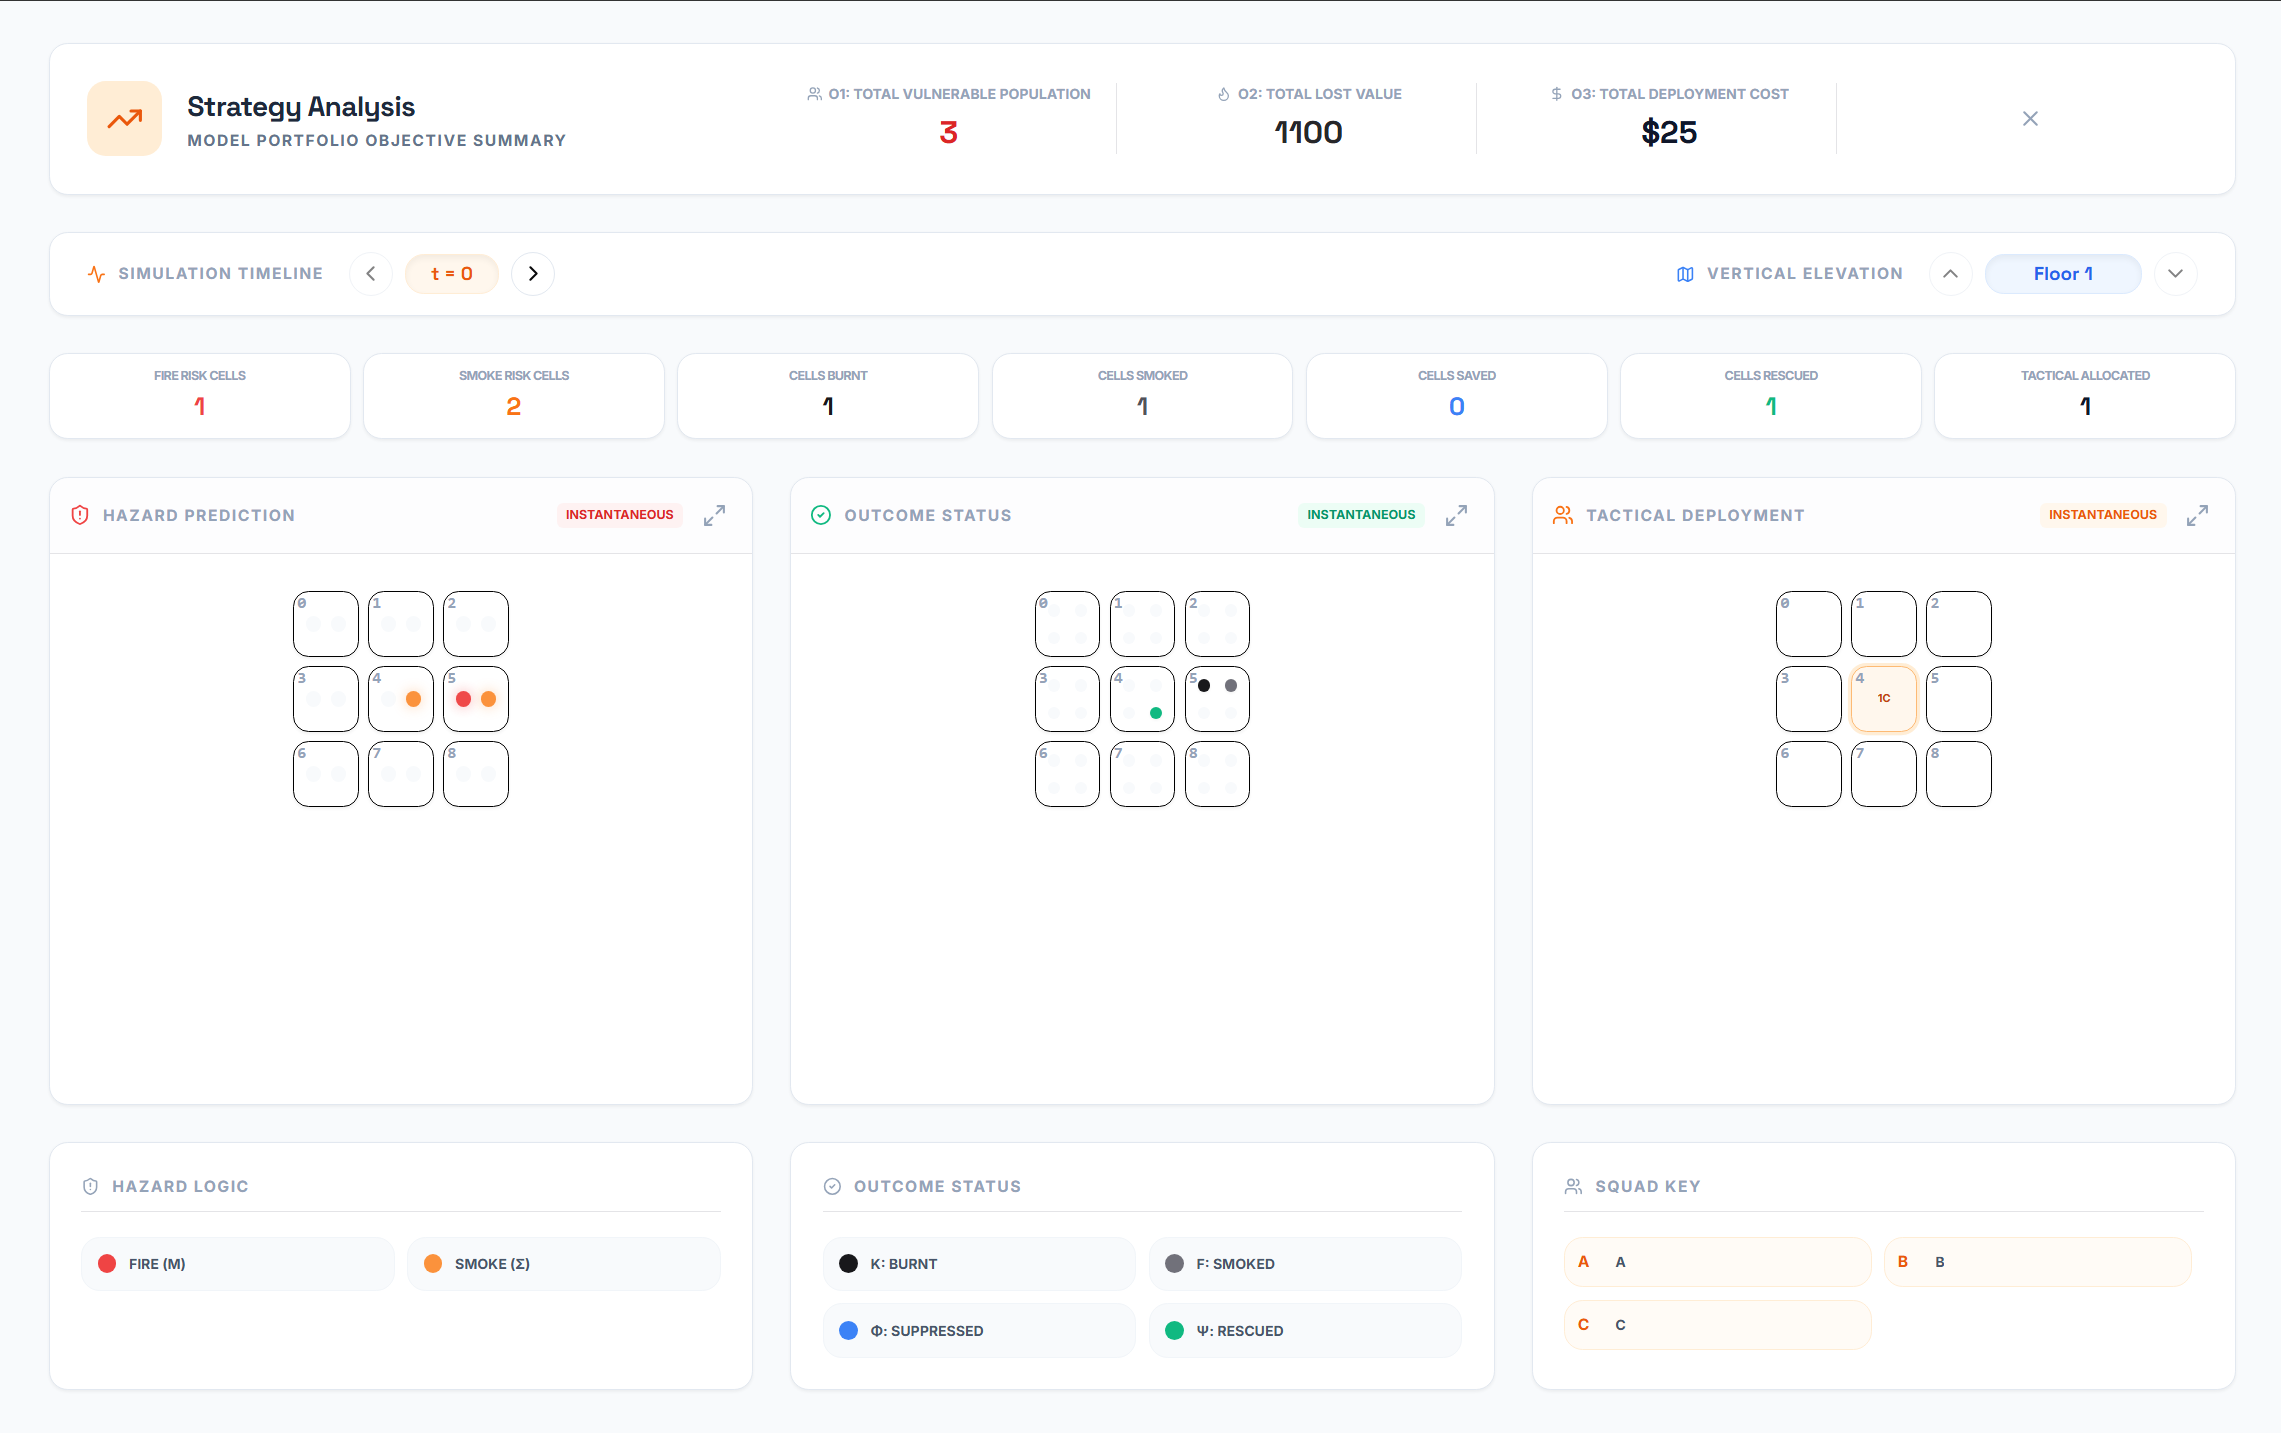
\includegraphics[width=0.32\textwidth]{figures/1t0.png}}
\hfil
\subfloat[$t=1$ Allocation]{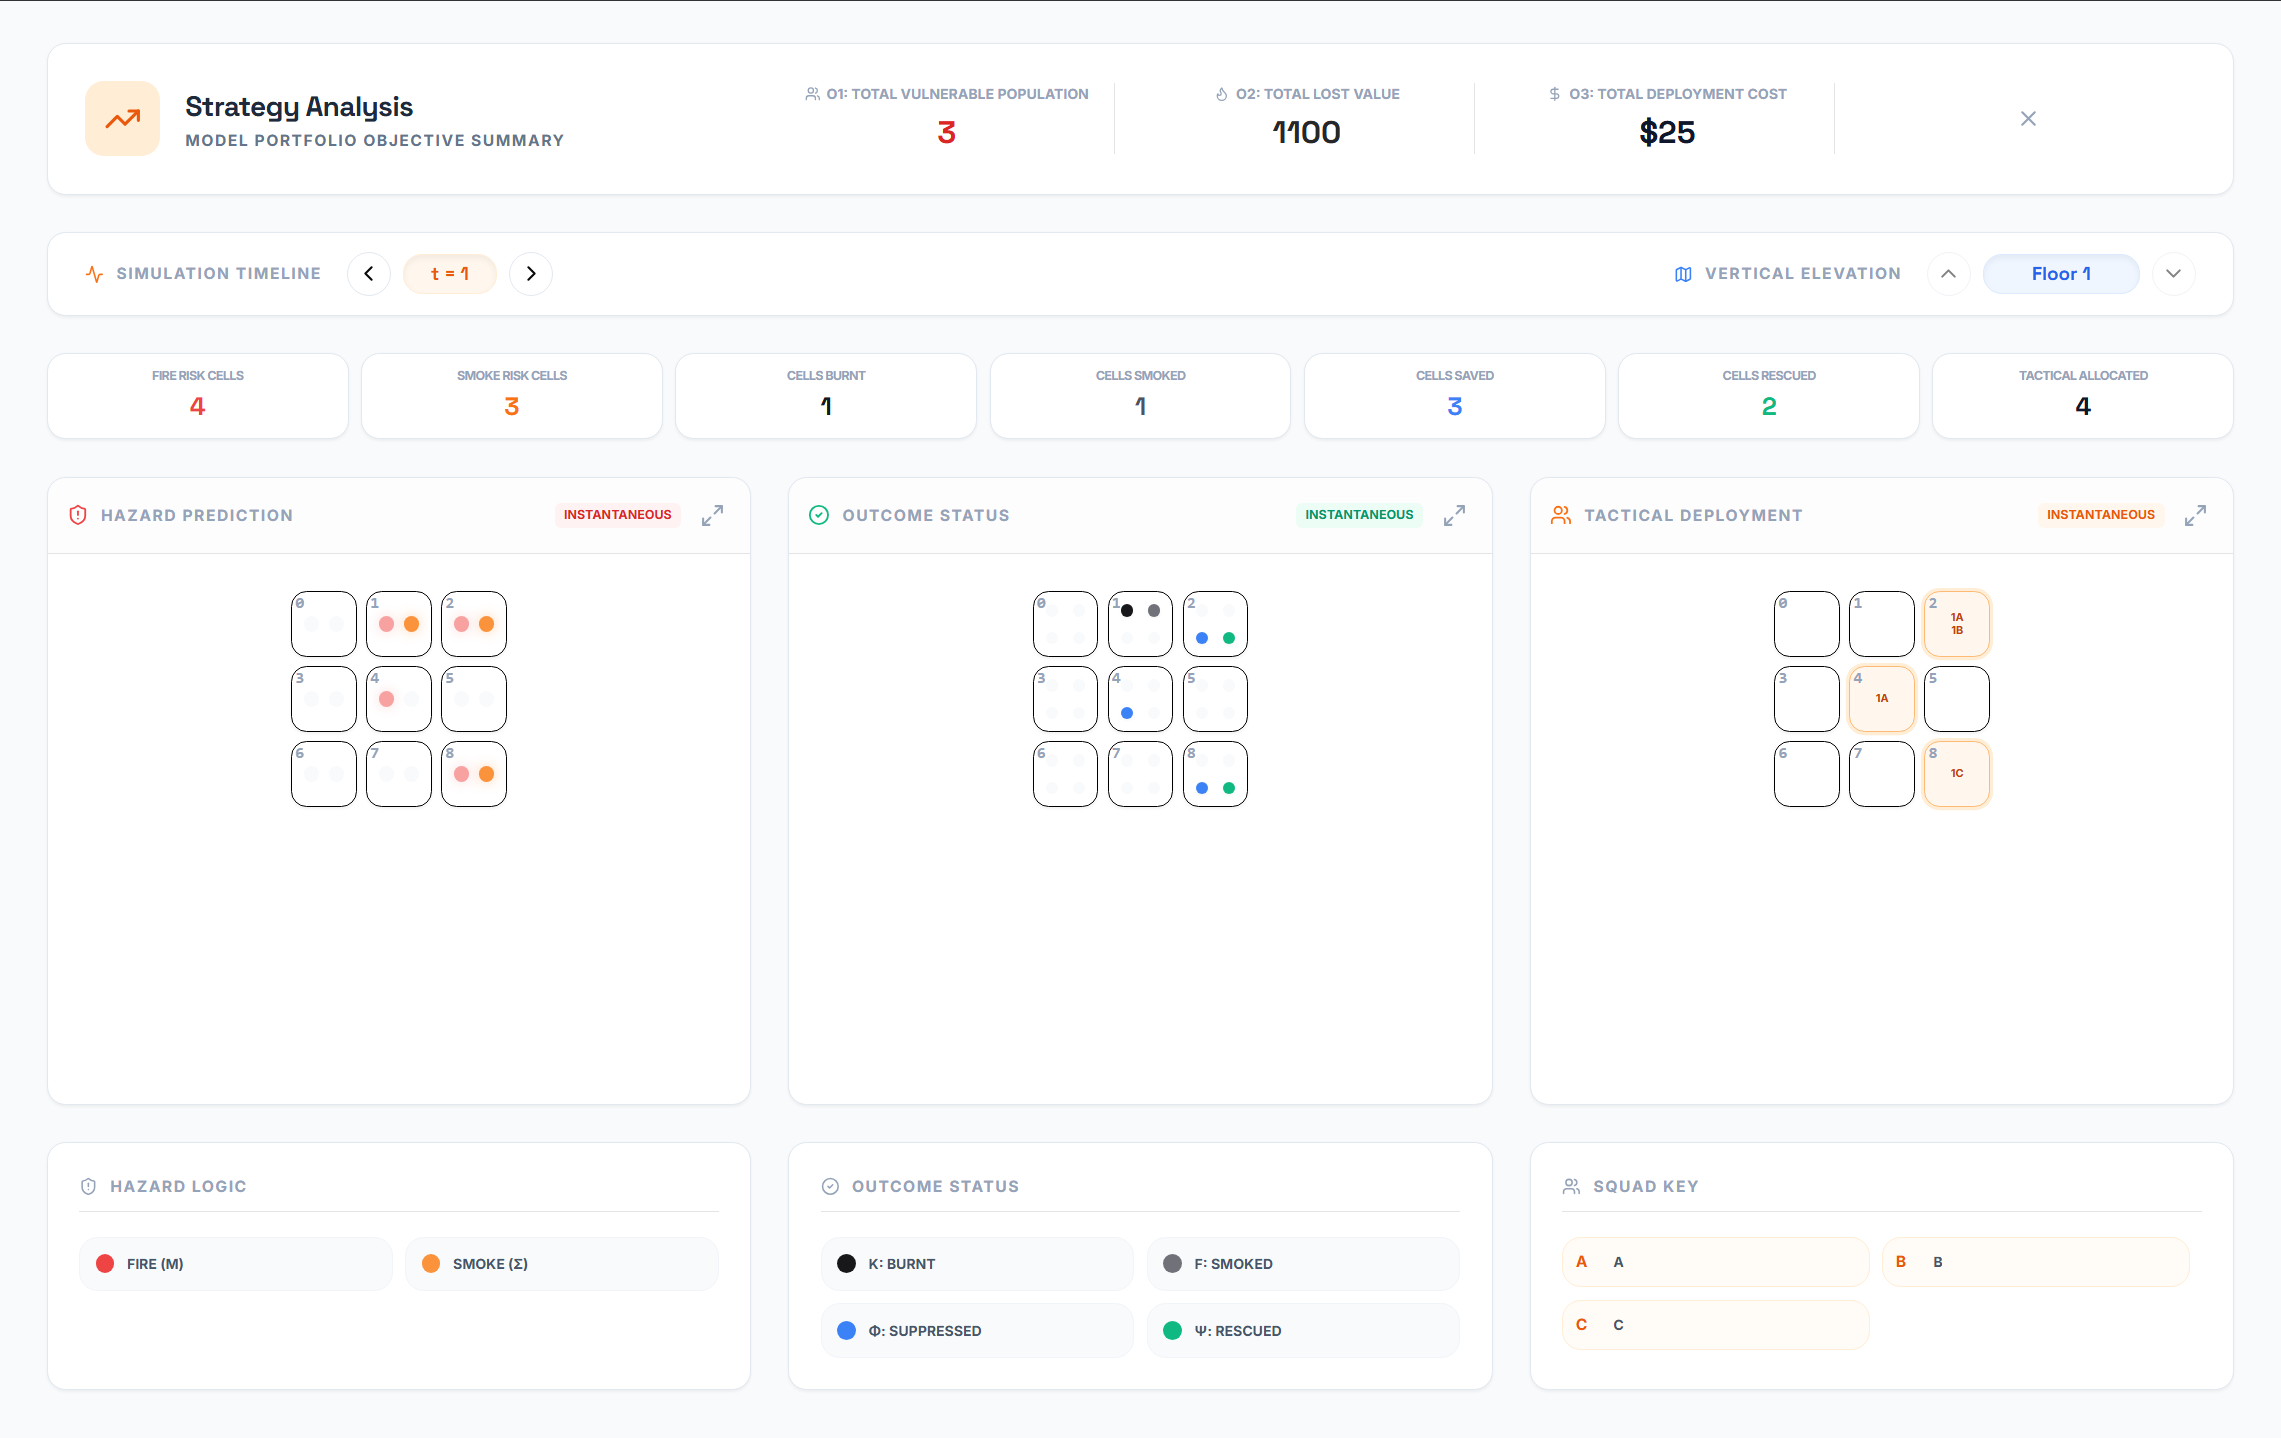
\includegraphics[width=0.32\textwidth]{figures/1t1.png}}
\hfil
\subfloat[$t=2$ Allocation]{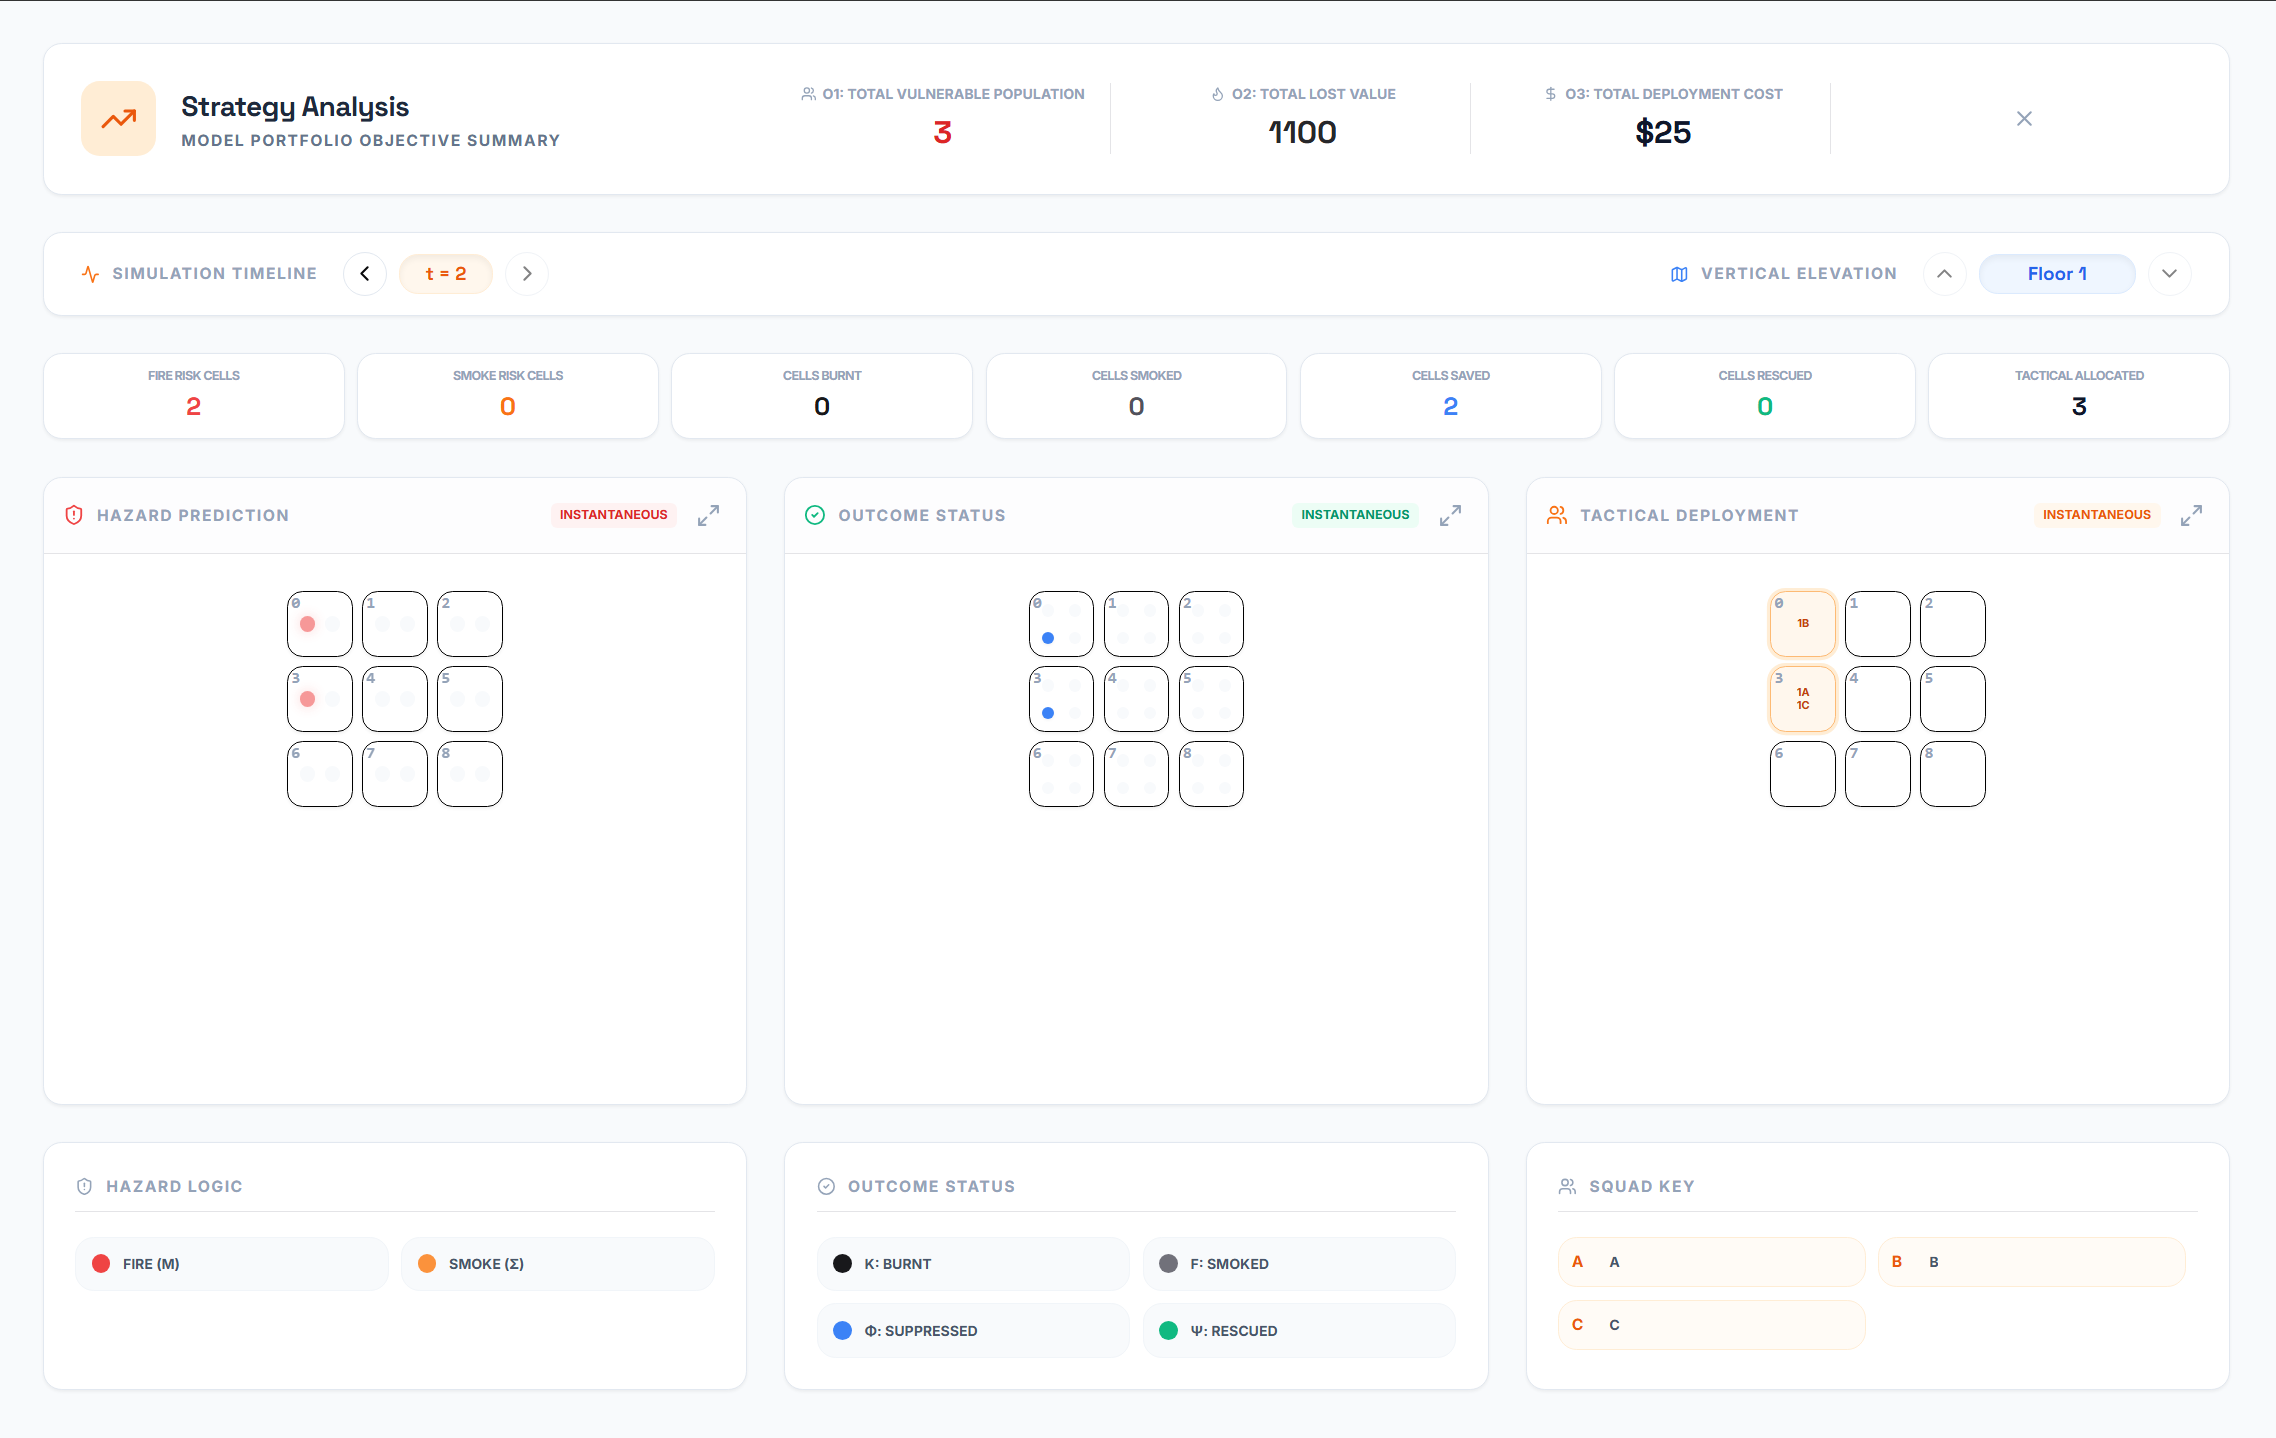
\includegraphics[width=0.32\textwidth]{figures/1t2.png}}
\caption{Simulation results across time steps showing hazard prediction, outcome status, and tactical deployment.}
\label{fig:sim_results}
\end{figure*}

\begin{figure*}[!htb]
\centering
\subfloat[Floor 0 Parameters]{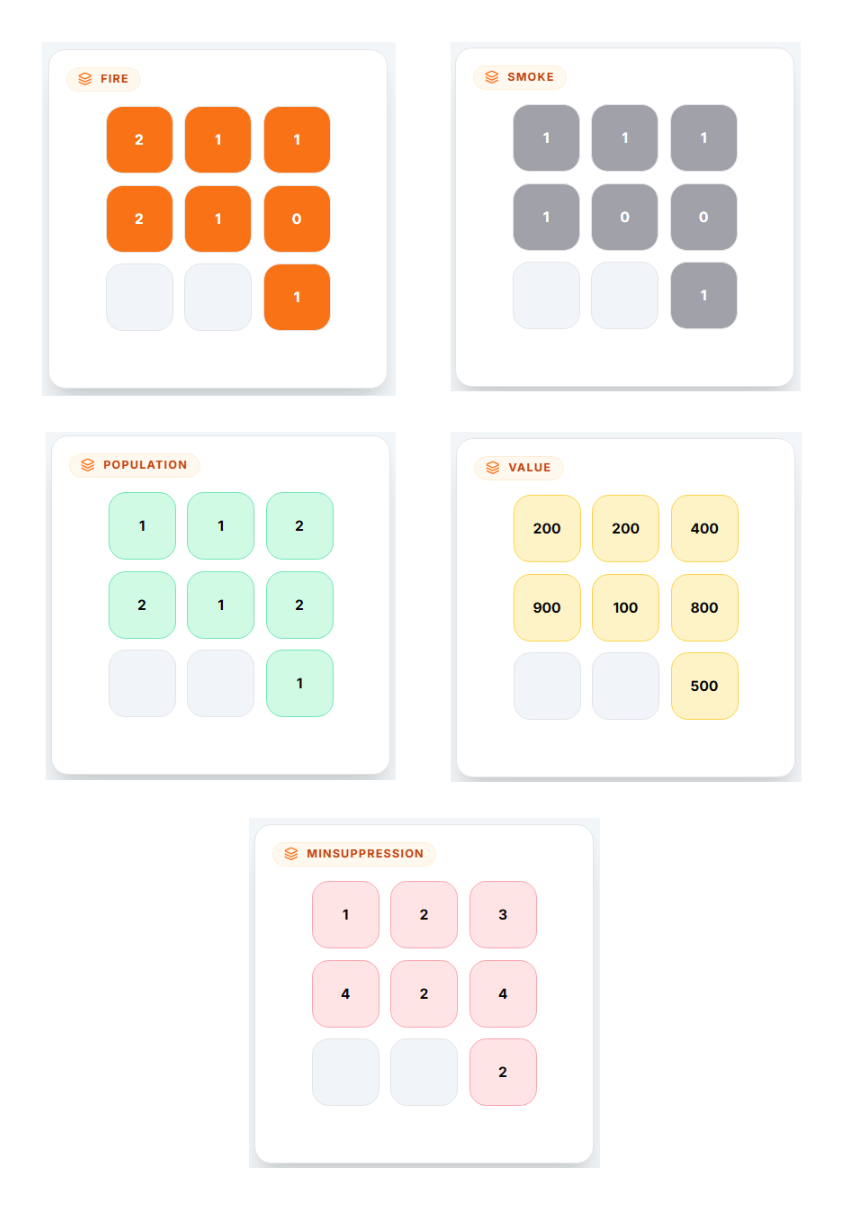
\includegraphics[width=0.45\textwidth]{figures/2floor1.png}}
\hfil
\subfloat[Floor 1 Parameters]{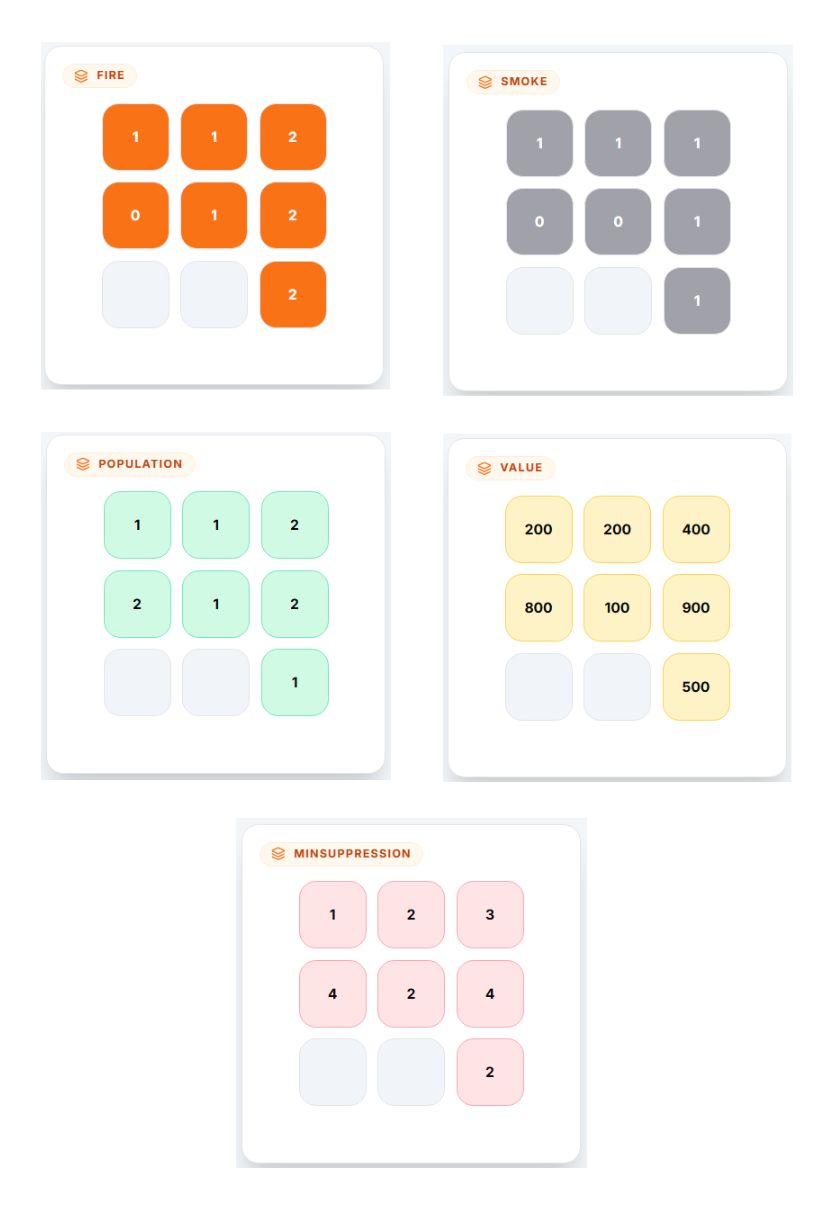
\includegraphics[width=0.45\textwidth]{figures/2floor2.png}}
\caption{Environmental parameters for the two-floor case study.}
\label{fig:case2_params}
\end{figure*}

\begin{figure*}[!htb]
\centering
\subfloat[$t=0$]{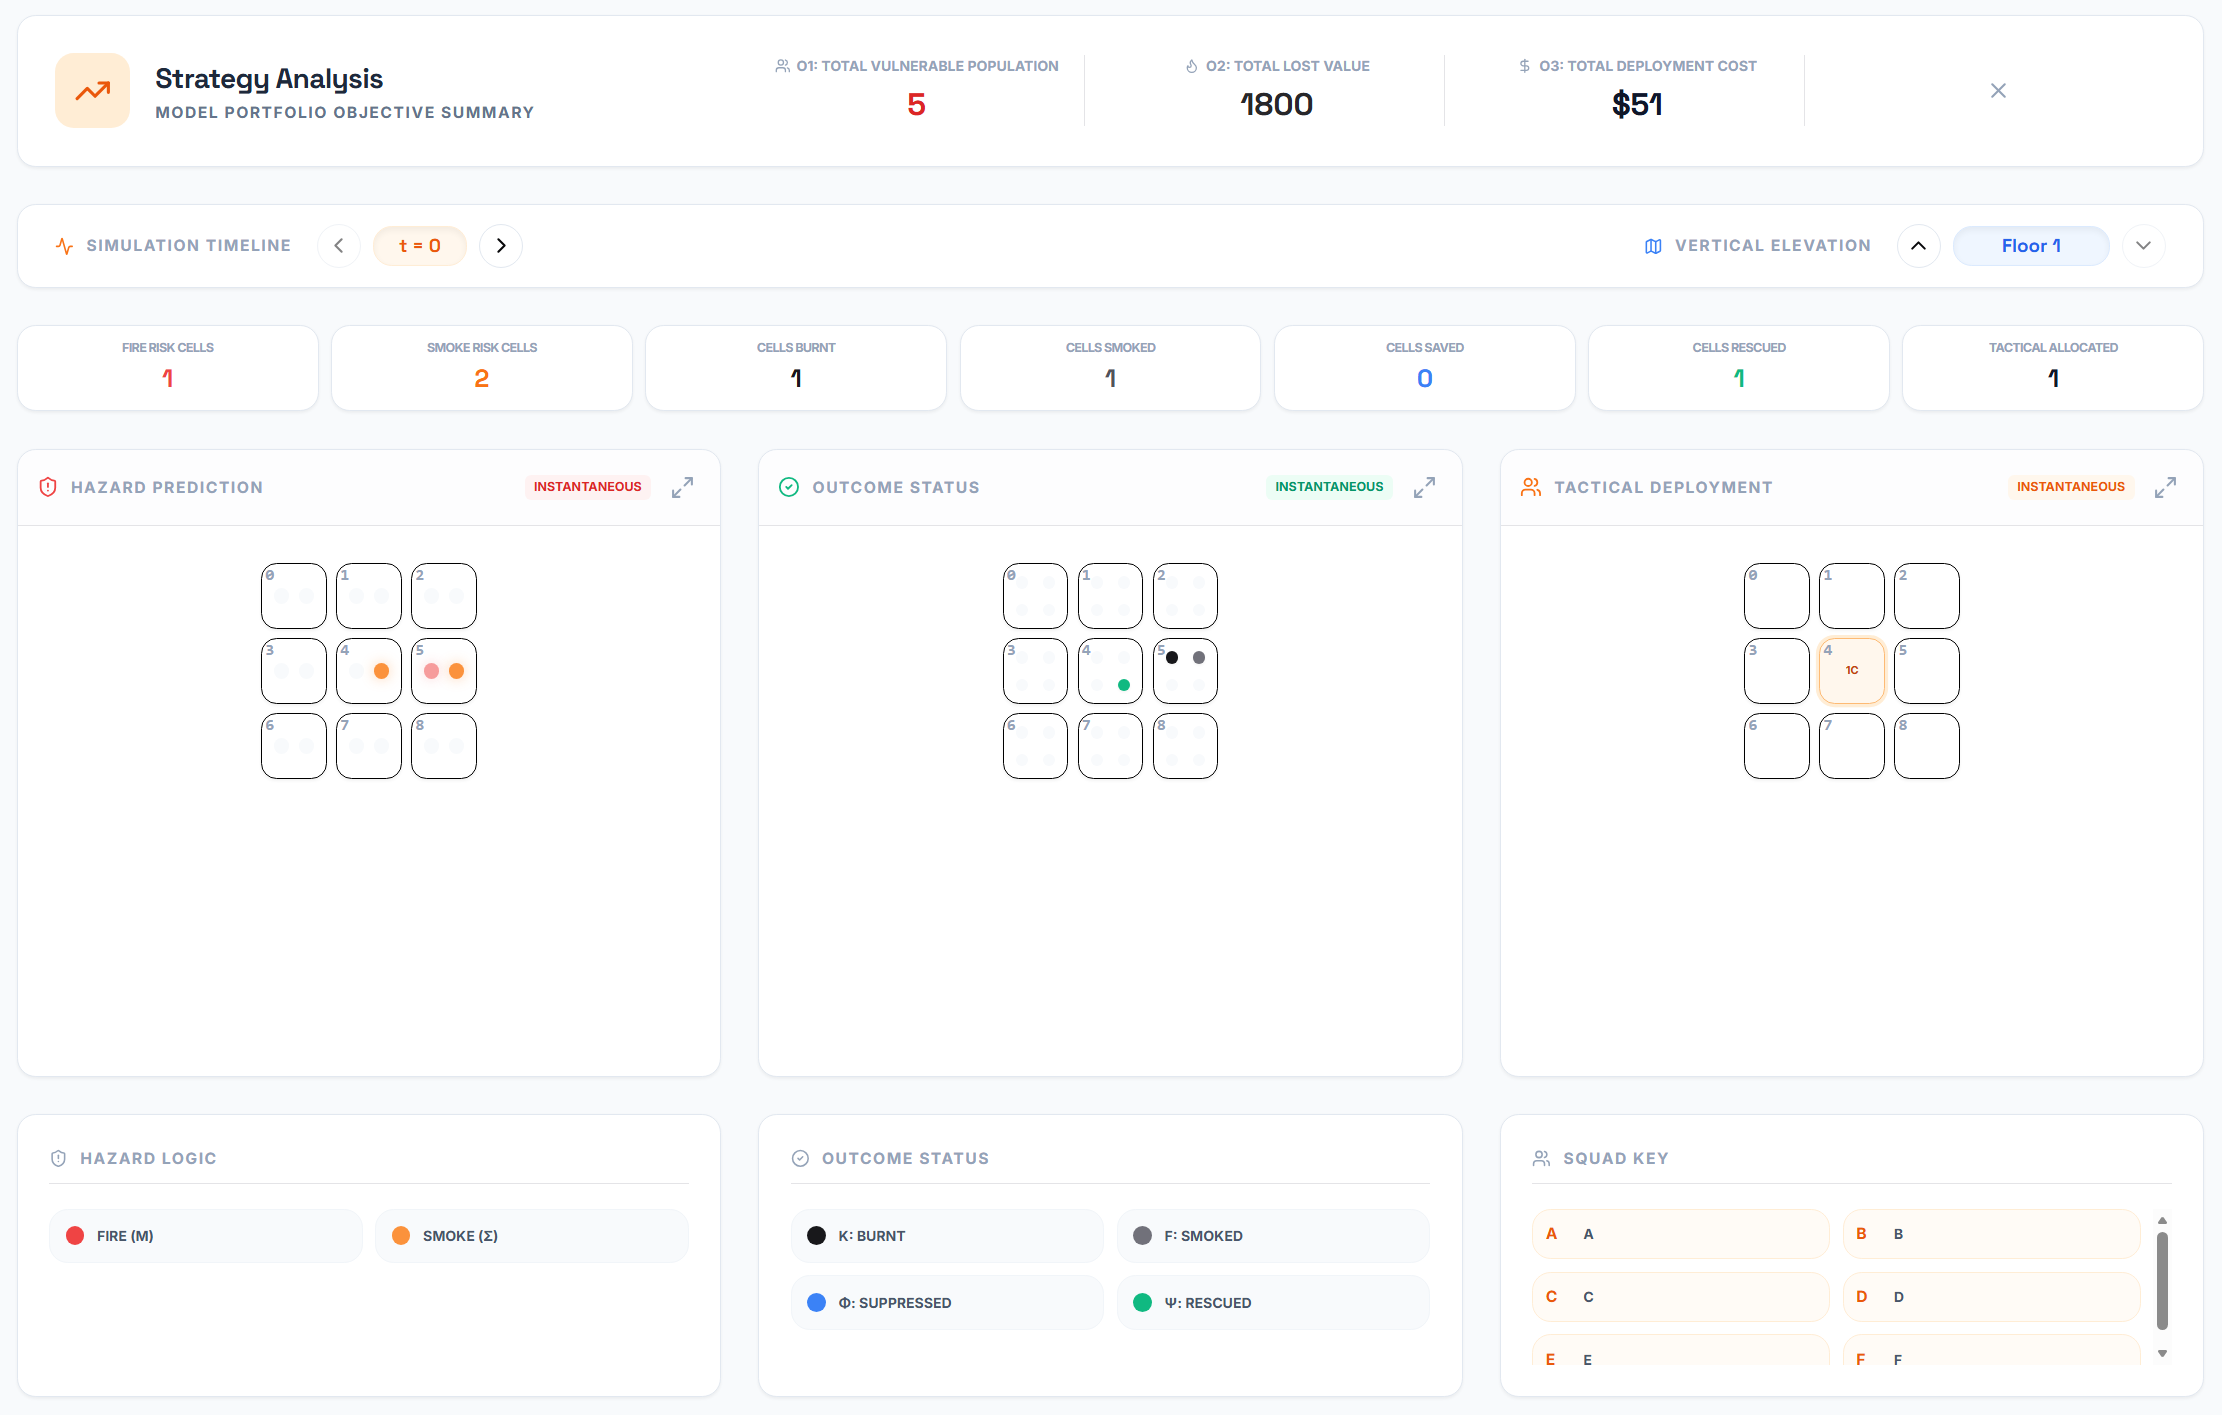
\includegraphics[width=0.32\textwidth]{figures/2t0f1.png}}
\hfil
\subfloat[$t=1$]{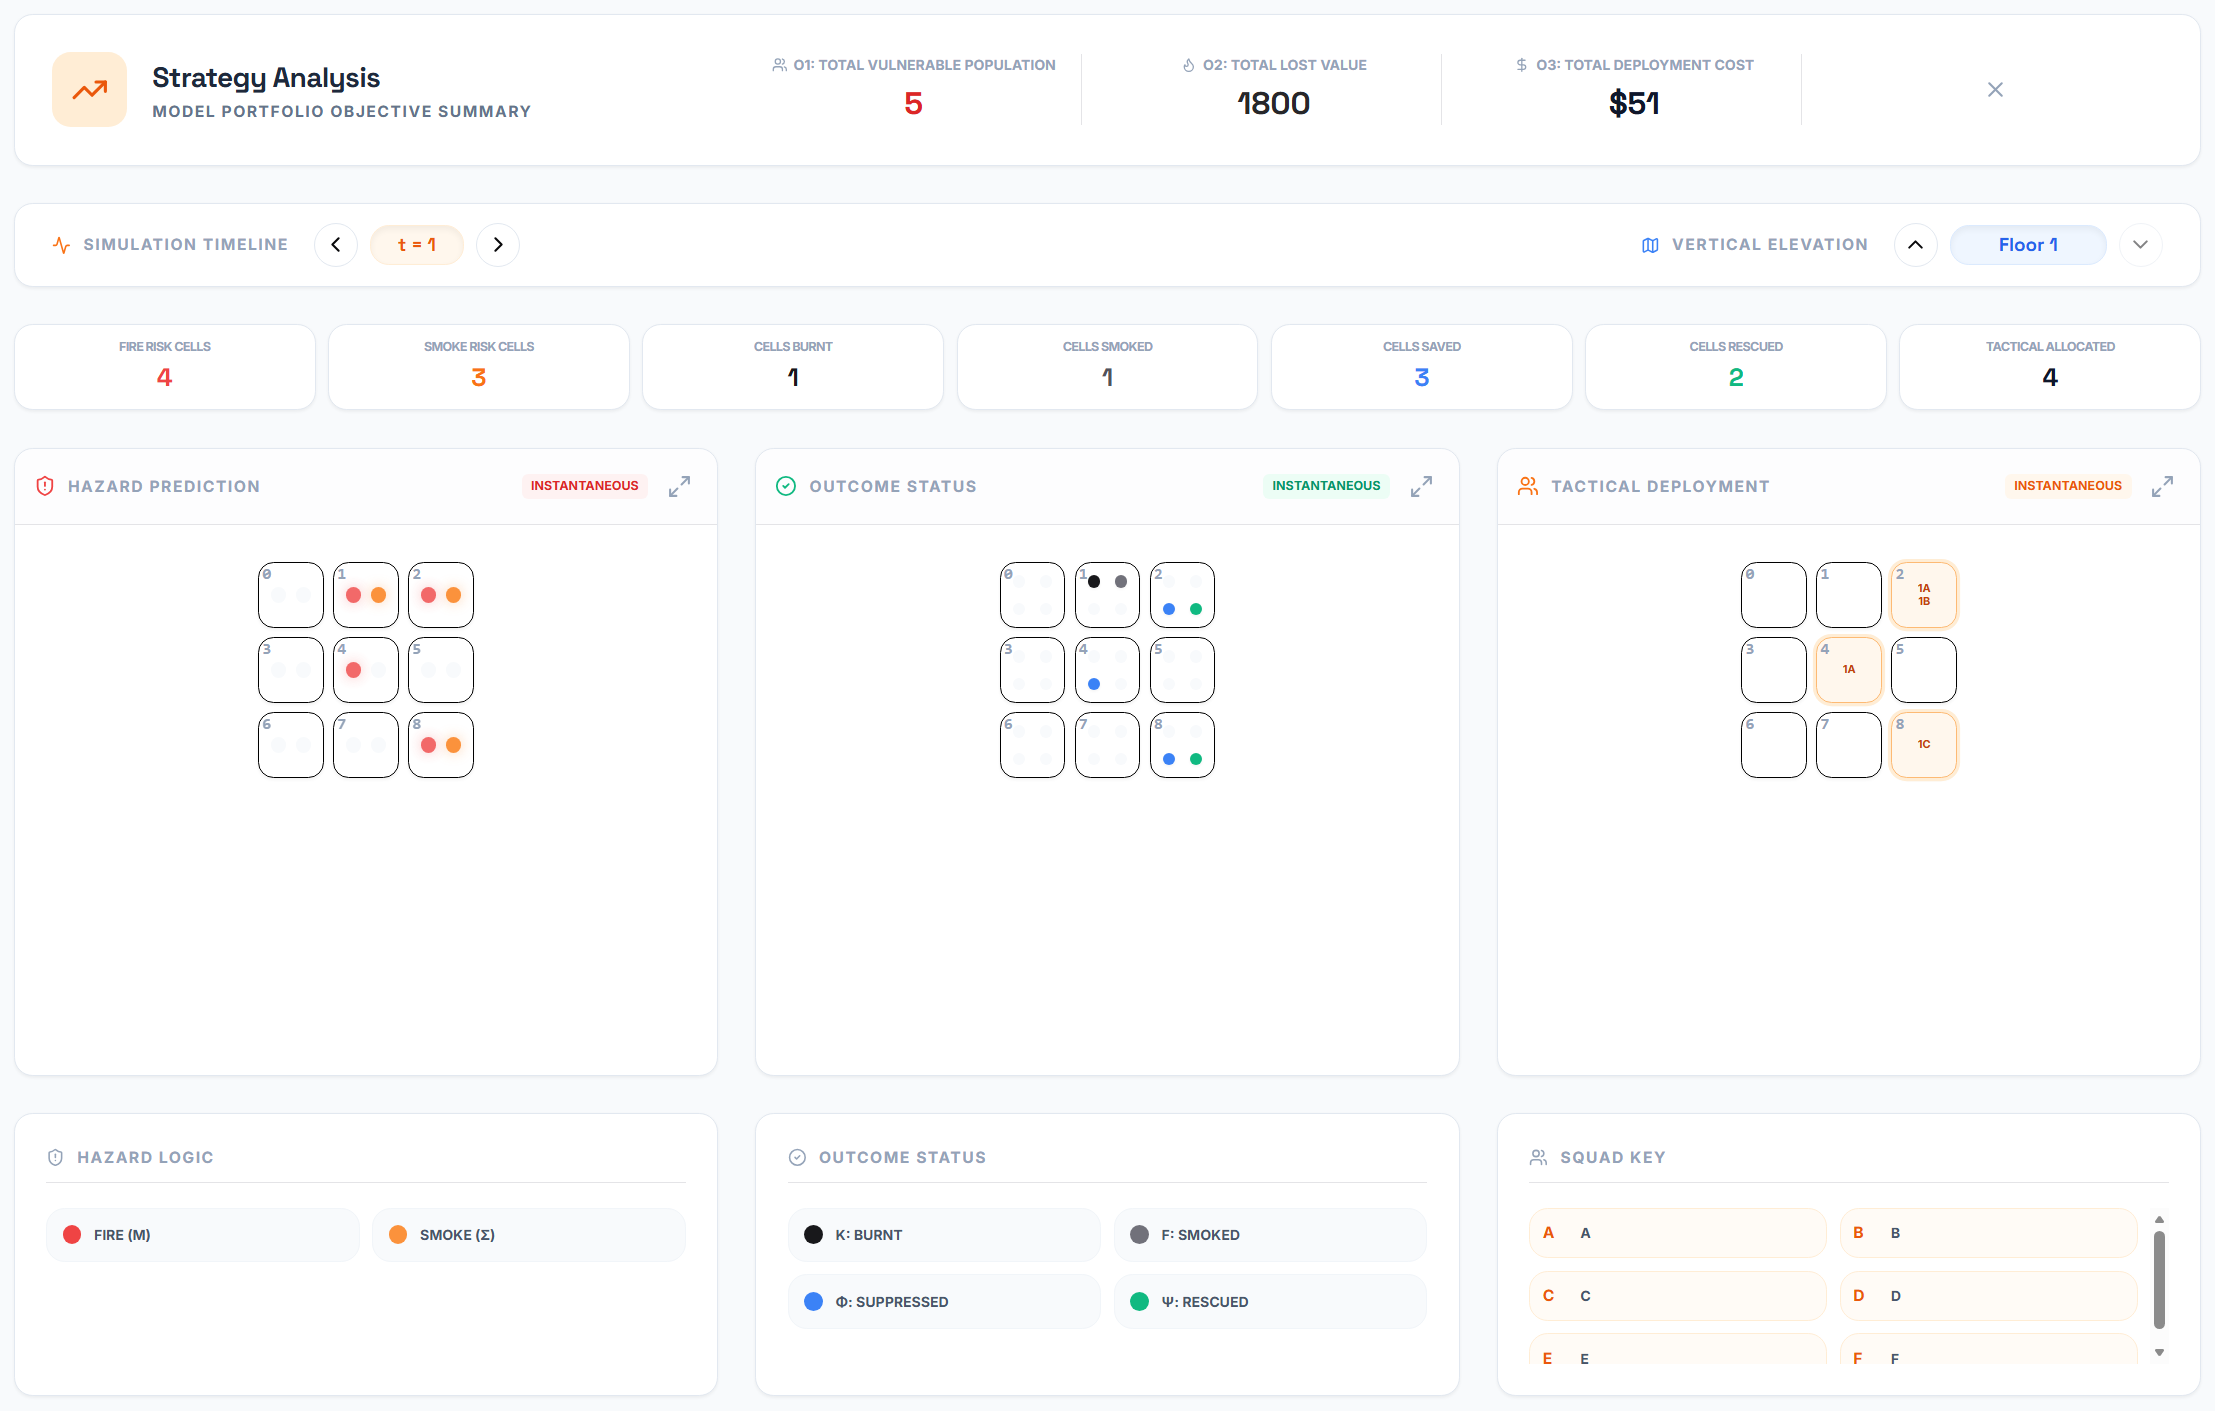
\includegraphics[width=0.32\textwidth]{figures/2t1f1.png}}
\hfil
\subfloat[$t=2$]{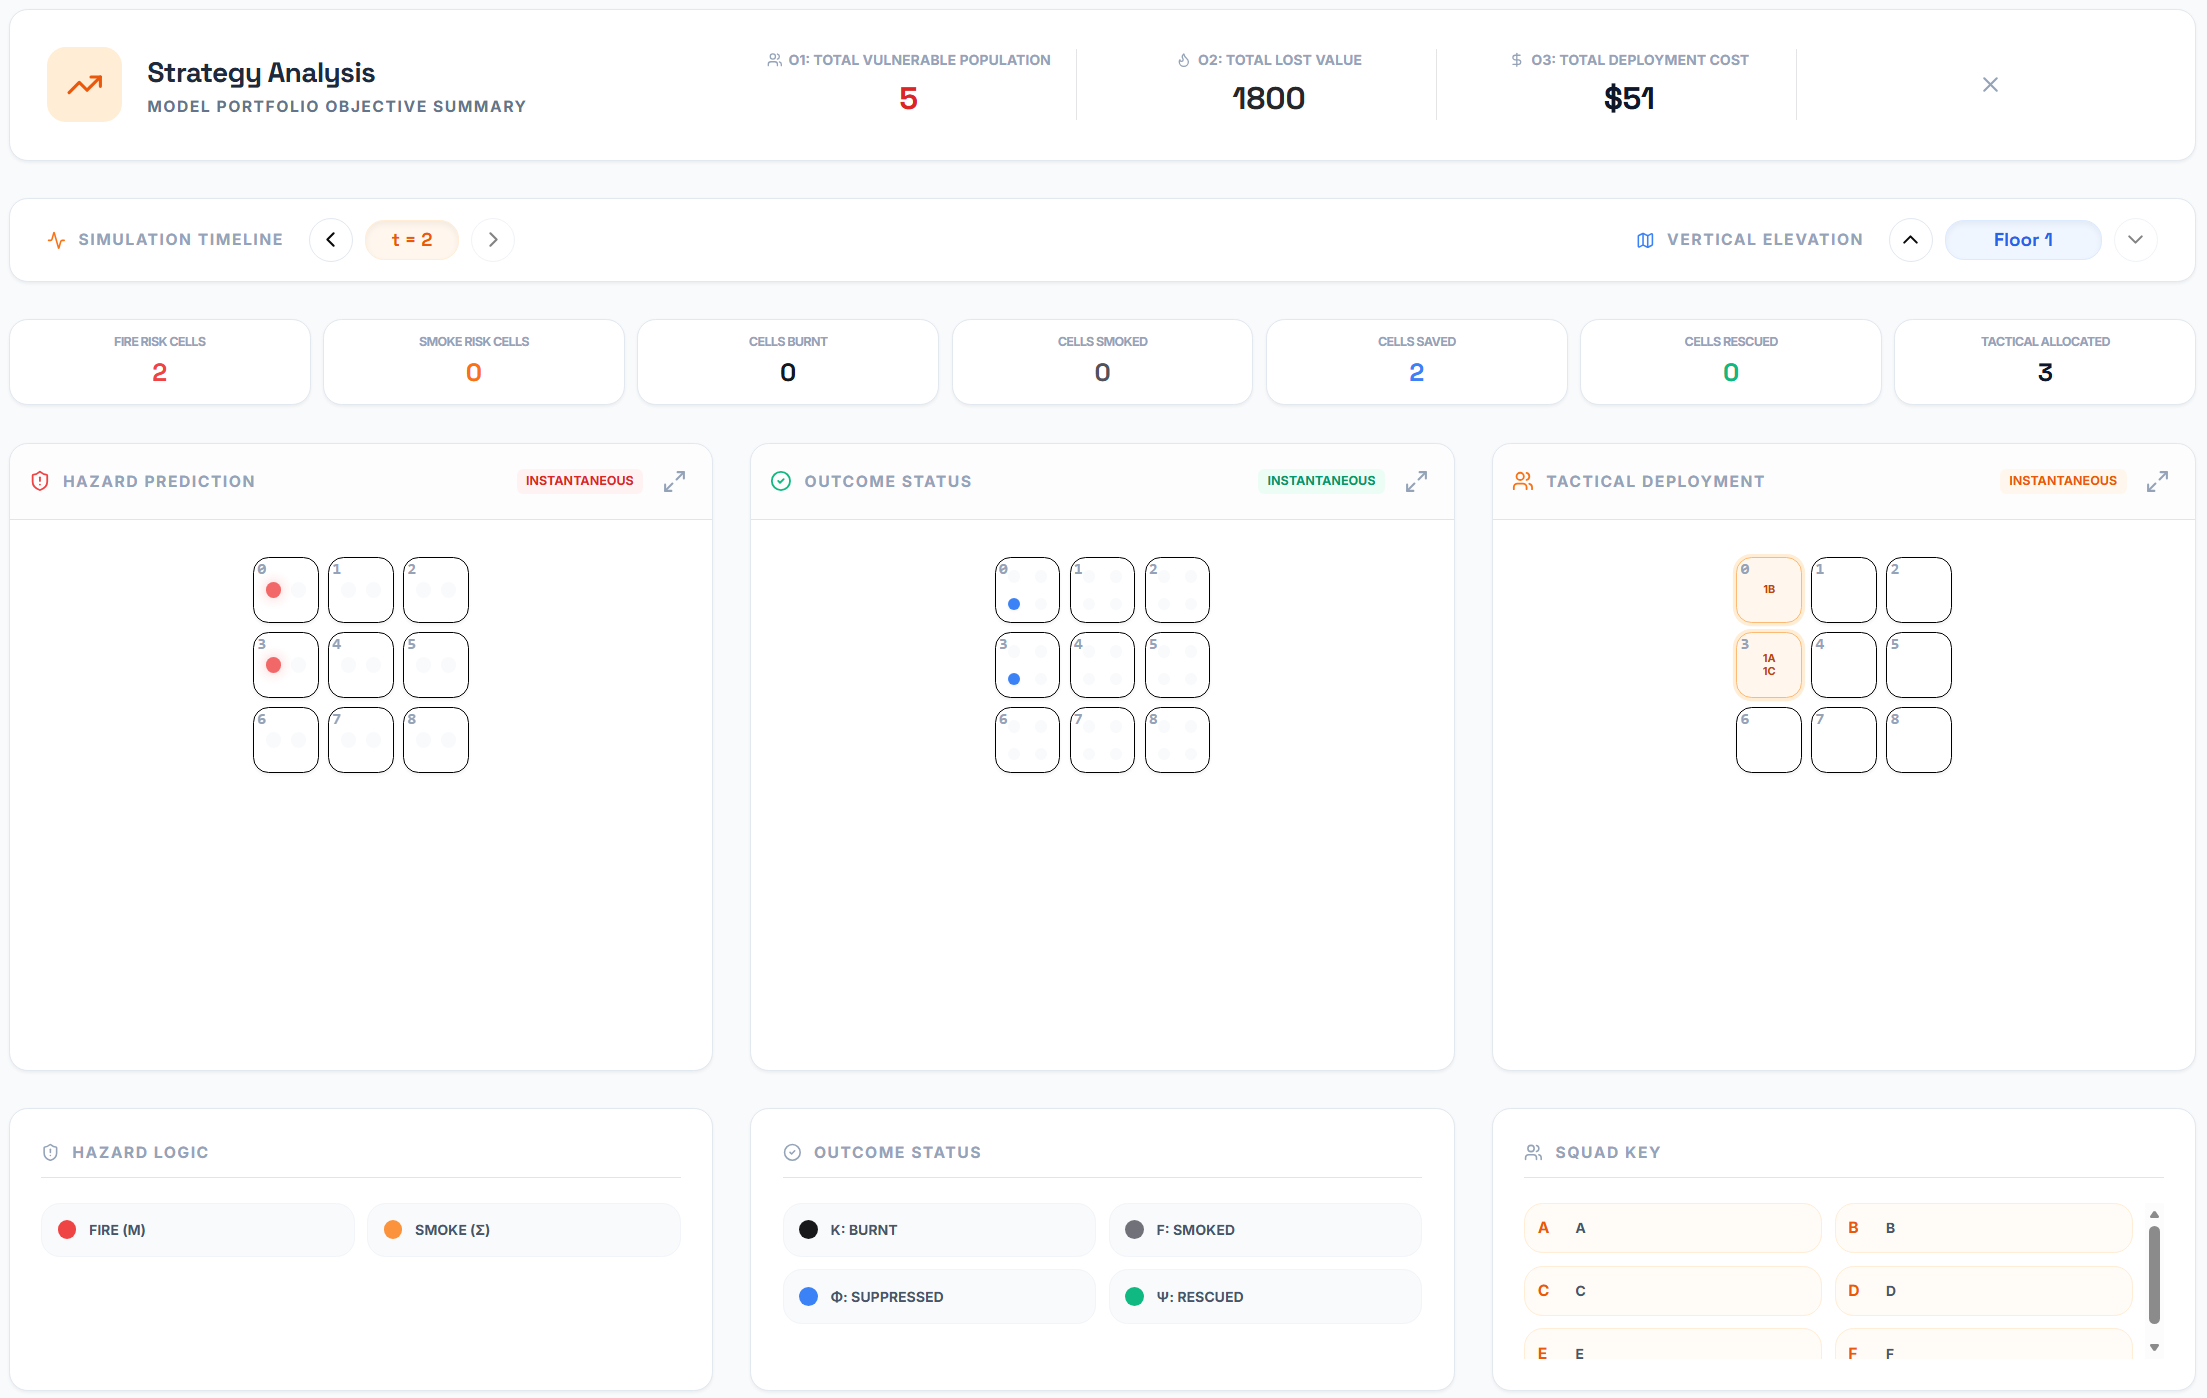
\includegraphics[width=0.32\textwidth]{figures/2t2f1.png}}
\caption{Simulation results for Floor 0 showing hazard prediction, outcome status, and tactical deployment across time.}
\label{fig:case2_results_floor0}
\end{figure*}

\begin{figure*}[!htb]
\centering
\subfloat[$t=0$]{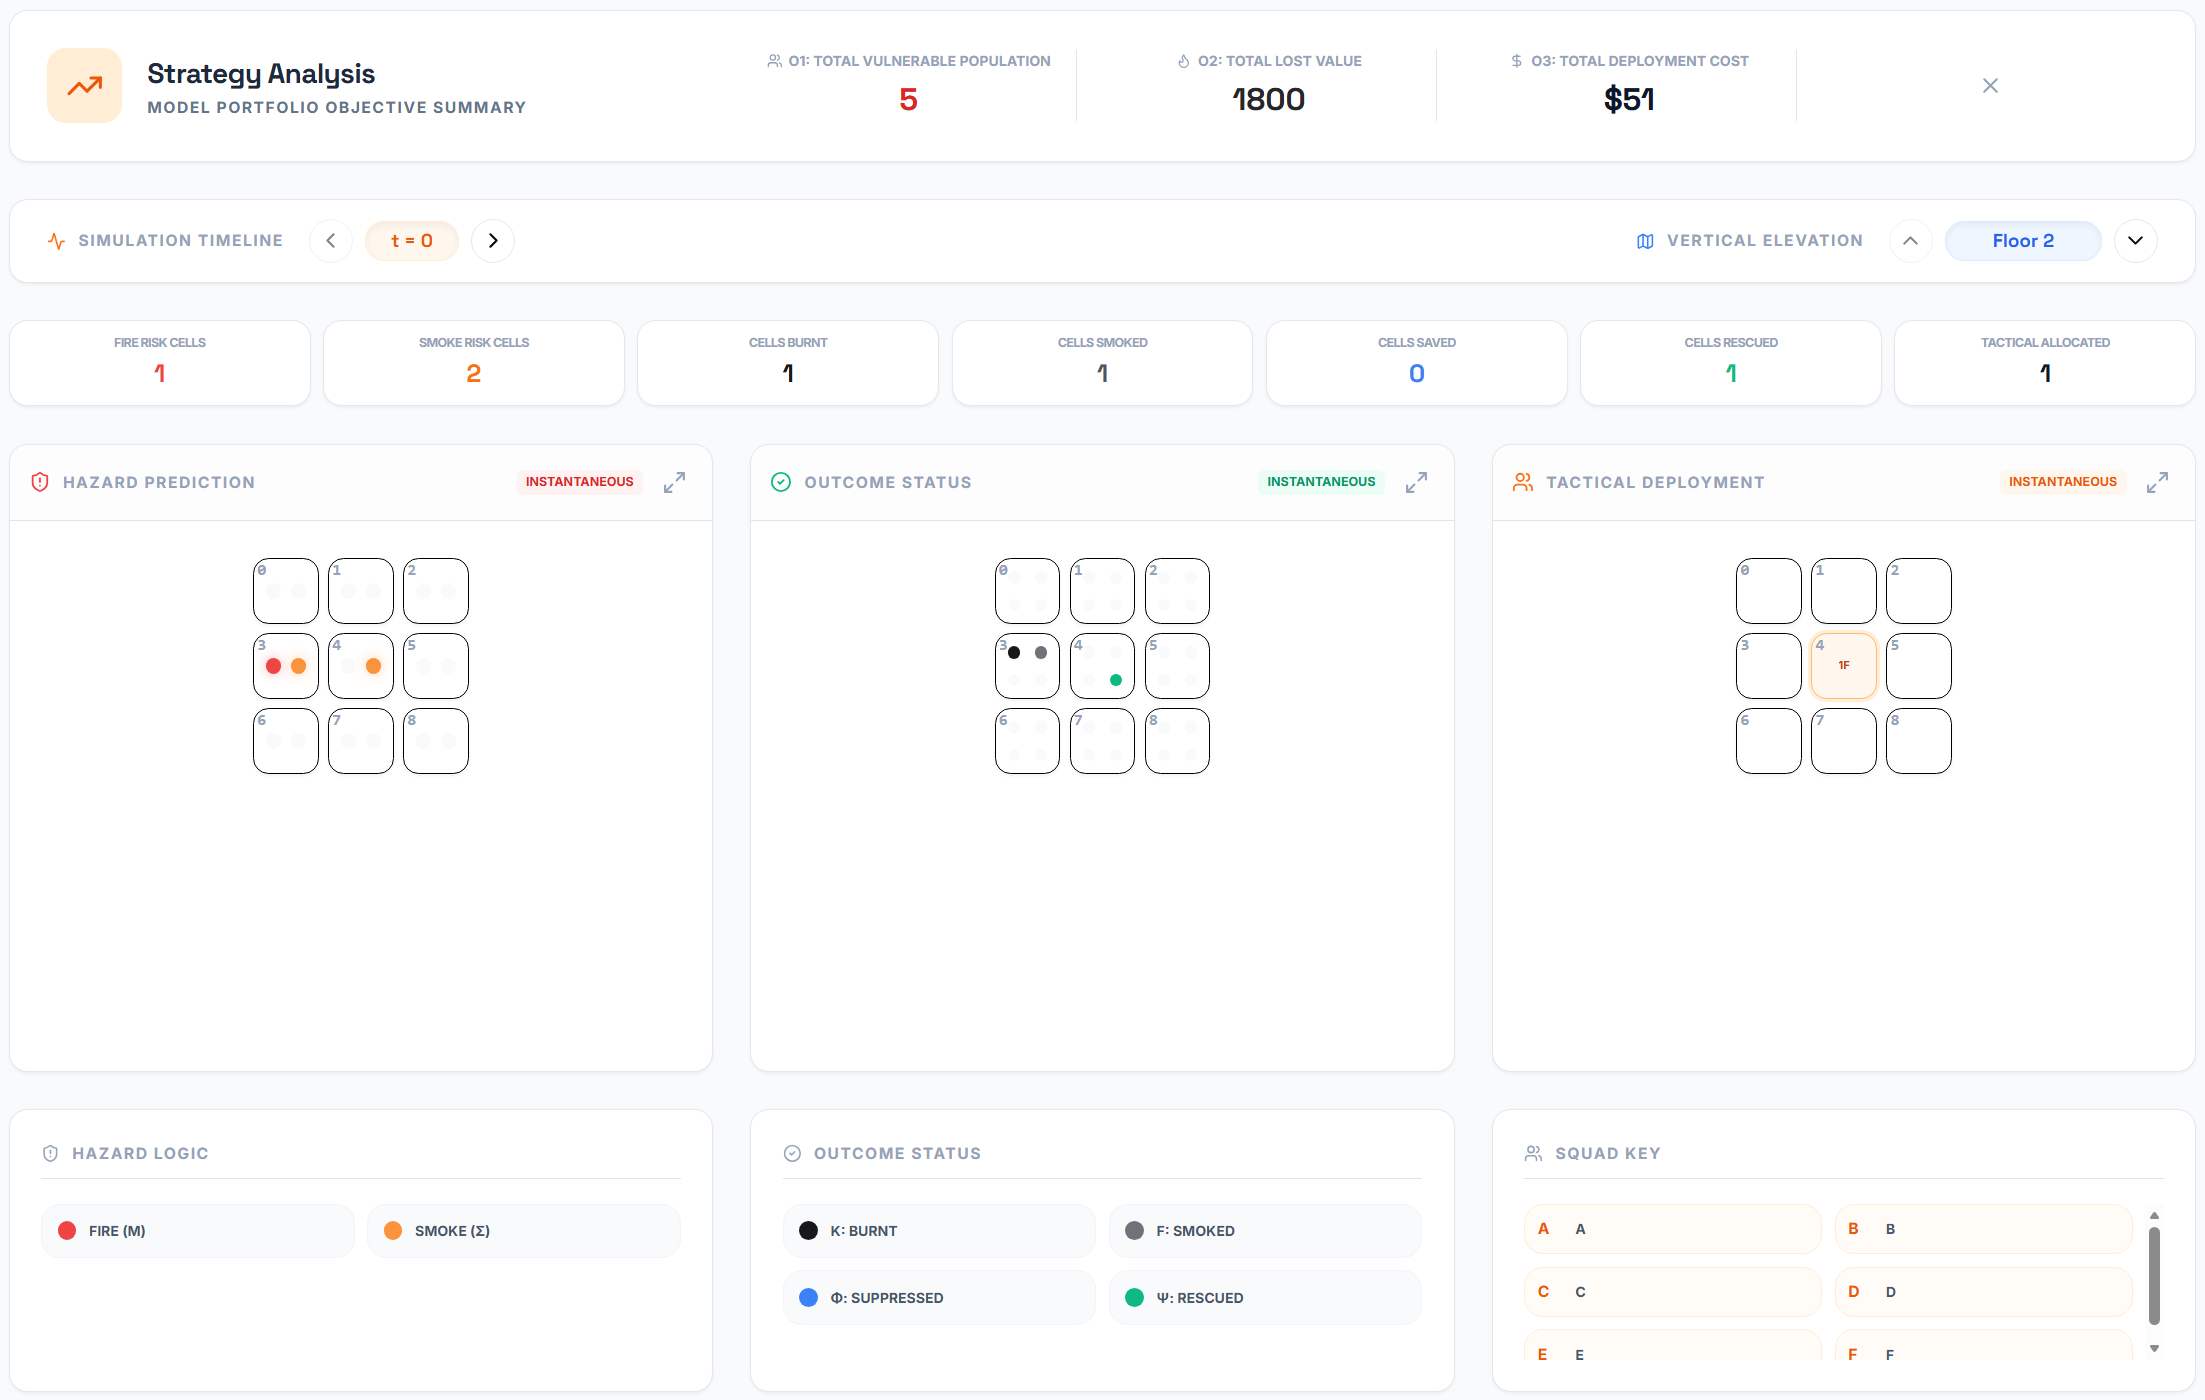
\includegraphics[width=0.32\textwidth]{figures/2t0f2.png}}
\hfil
\subfloat[$t=1$]{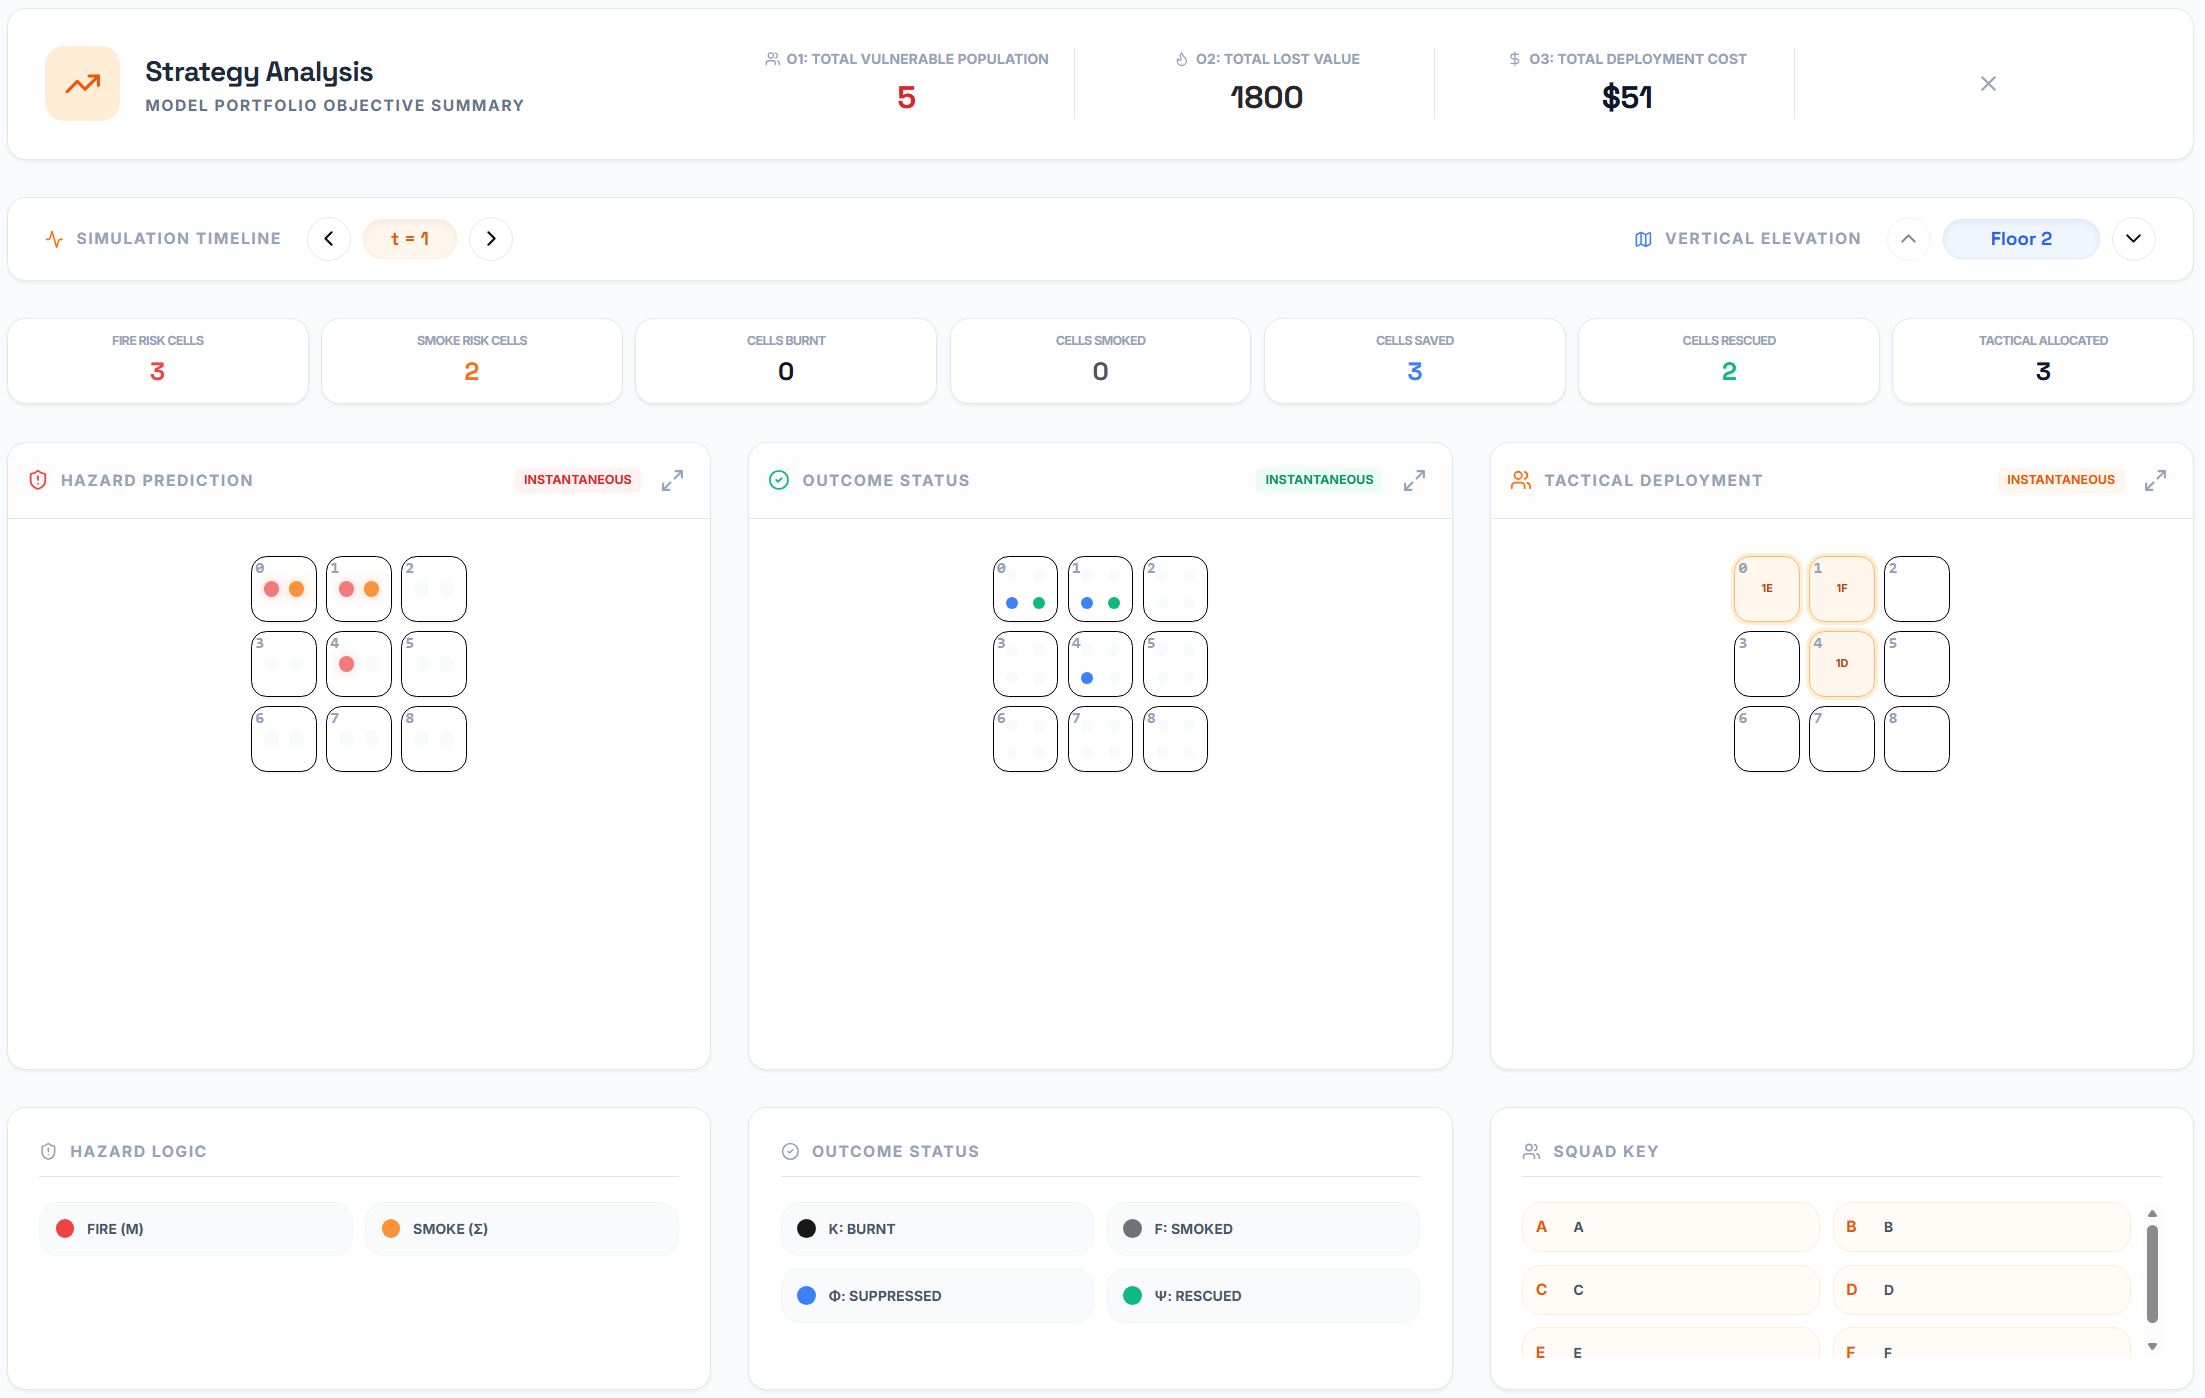
\includegraphics[width=0.32\textwidth]{figures/2t1f2.png}}
\hfil
\subfloat[$t=2$]{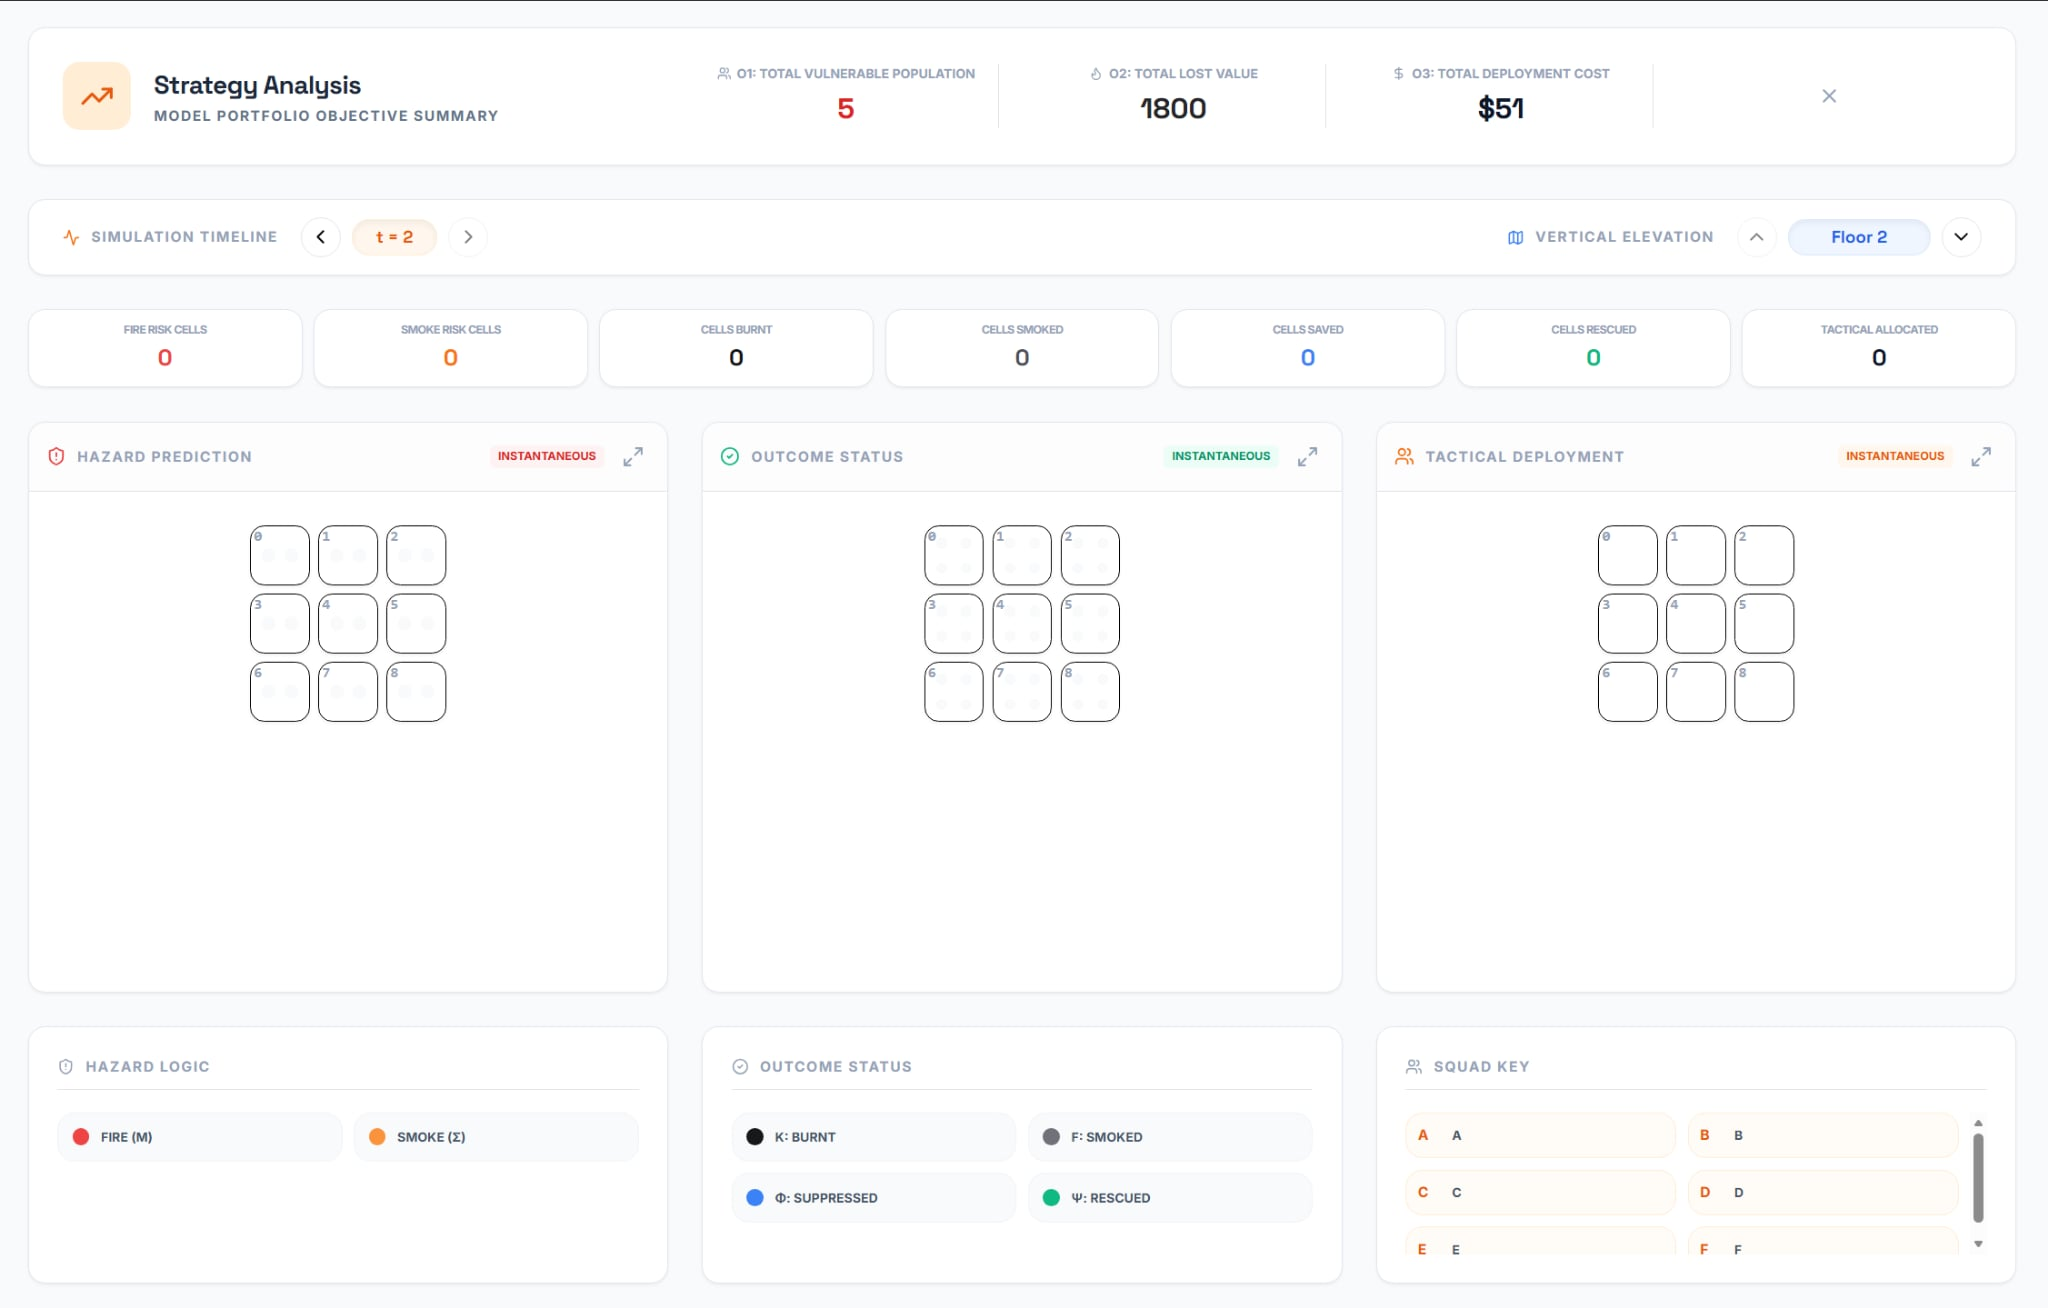
\includegraphics[width=0.32\textwidth]{figures/2t2f2.png}}
\caption{Simulation results for Floor 1 showing hazard prediction, outcome status, and tactical deployment across time.}
\label{fig:case2_results_floor1}
\end{figure*}

\begin{figure*}[!htb]
\centering
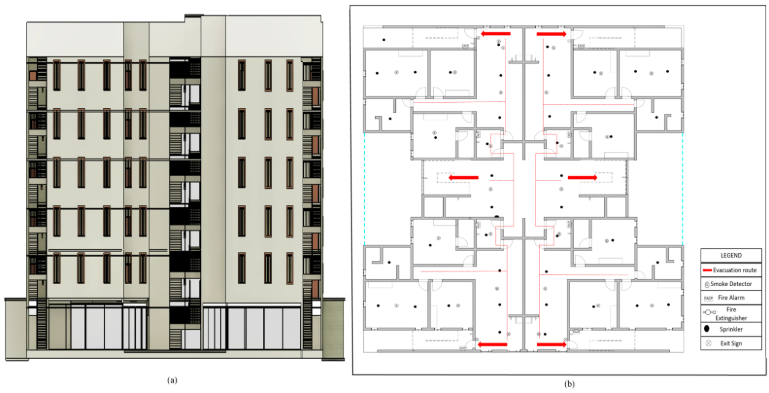
\includegraphics[width=\textwidth]{figures/building.png}  % ← changed to \textwidth for better scaling
\caption{Building layout used for the simulation scenario.}
\label{fig:building-layout}
\end{figure*}

\begin{figure*}[!htb]
\centering
\subfloat[Fire Arrival Time]{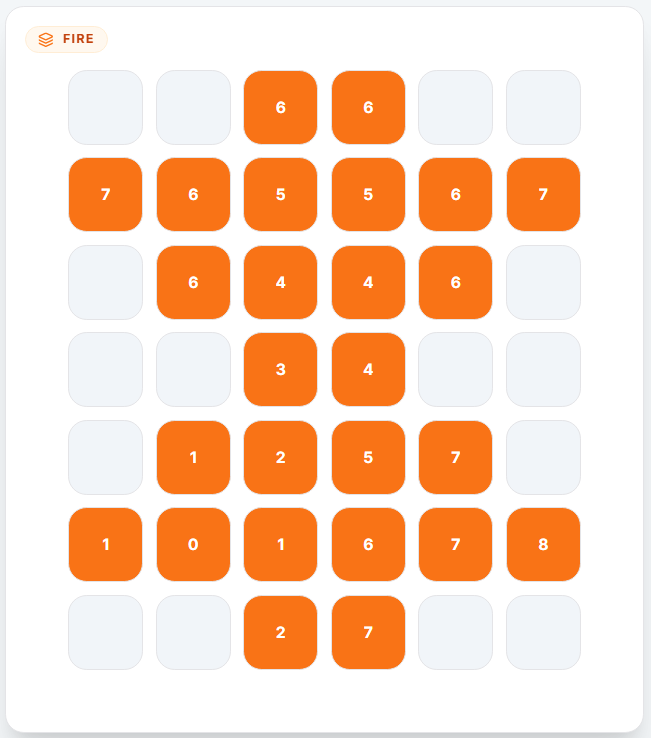
\includegraphics[width=0.18\textwidth]{figures/3fire.png}}
\hfil
\subfloat[Smoke Arrival Time]{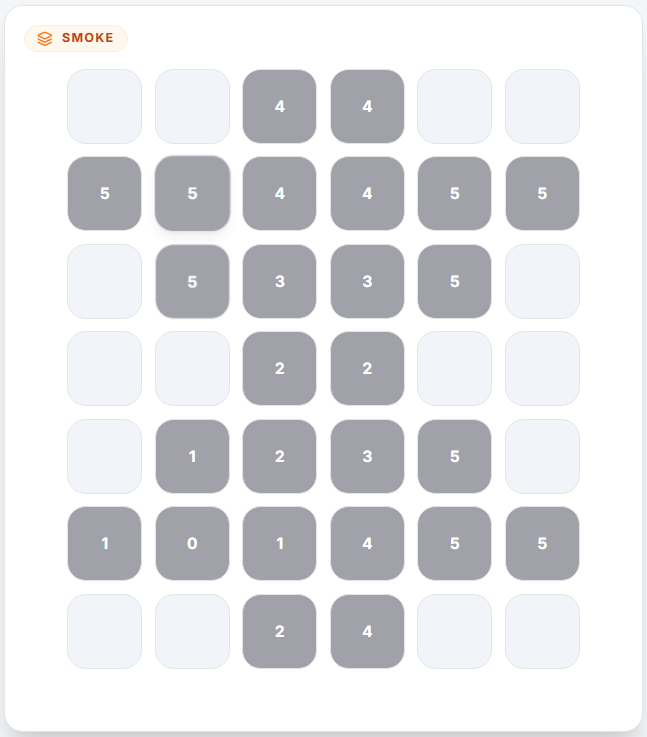
\includegraphics[width=0.18\textwidth]{figures/3smoke.png}}
\hfil
\subfloat[Population Distribution]{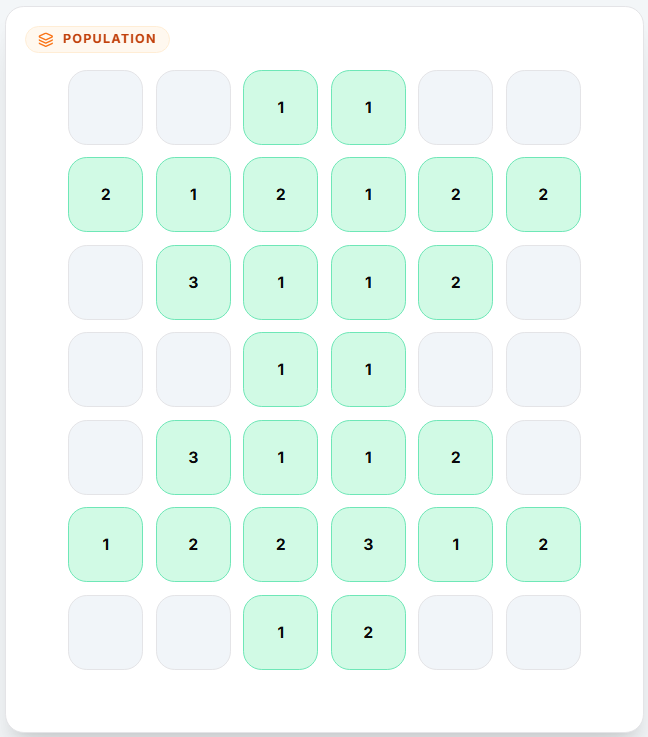
\includegraphics[width=0.18\textwidth]{figures/3population.png}}
\hfil
\subfloat[Property Value]{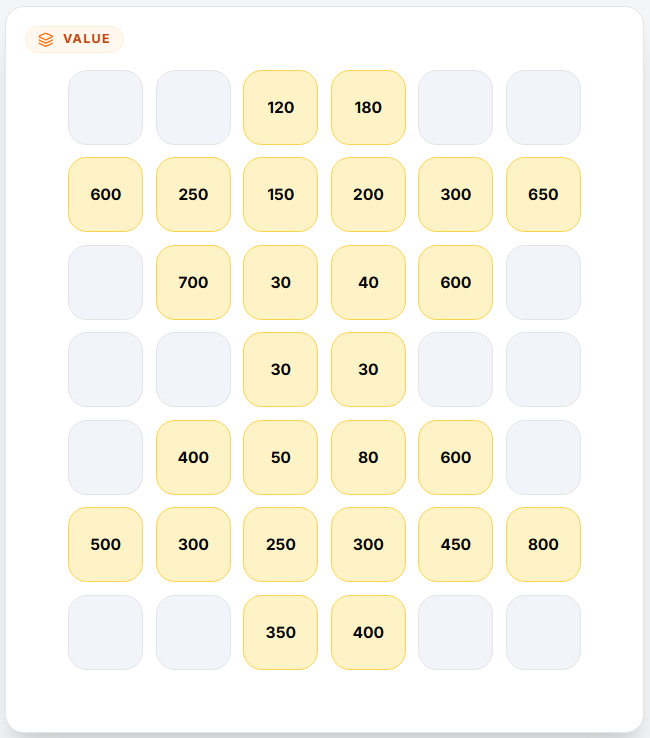
\includegraphics[width=0.18\textwidth]{figures/3value.png}}
\hfil
\subfloat[Min. Suppression]{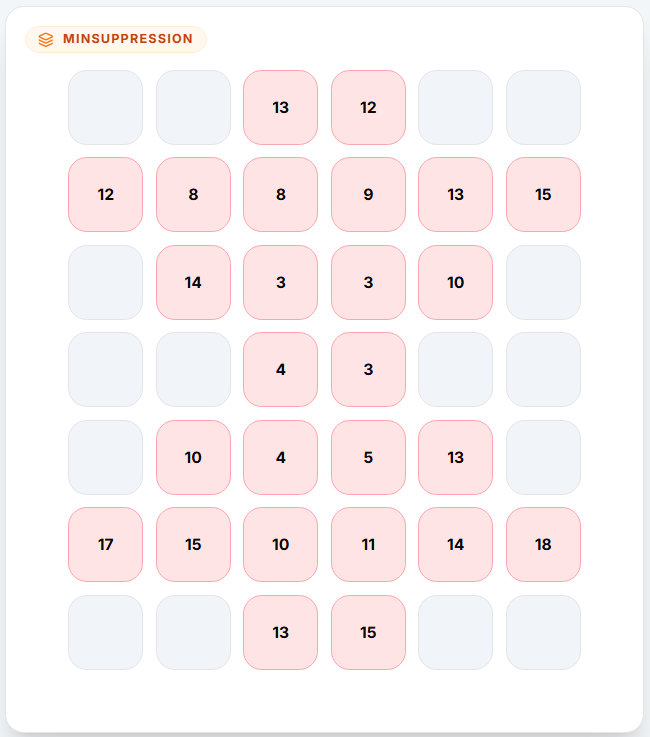
\includegraphics[width=0.18\textwidth]{figures/3min.png}}
\caption{Input matrices for the validation scenario.}
\label{fig:input-matrices}
\end{figure*}

\begin{figure*}[!htb]
\centering
\subfloat[$t=0$]{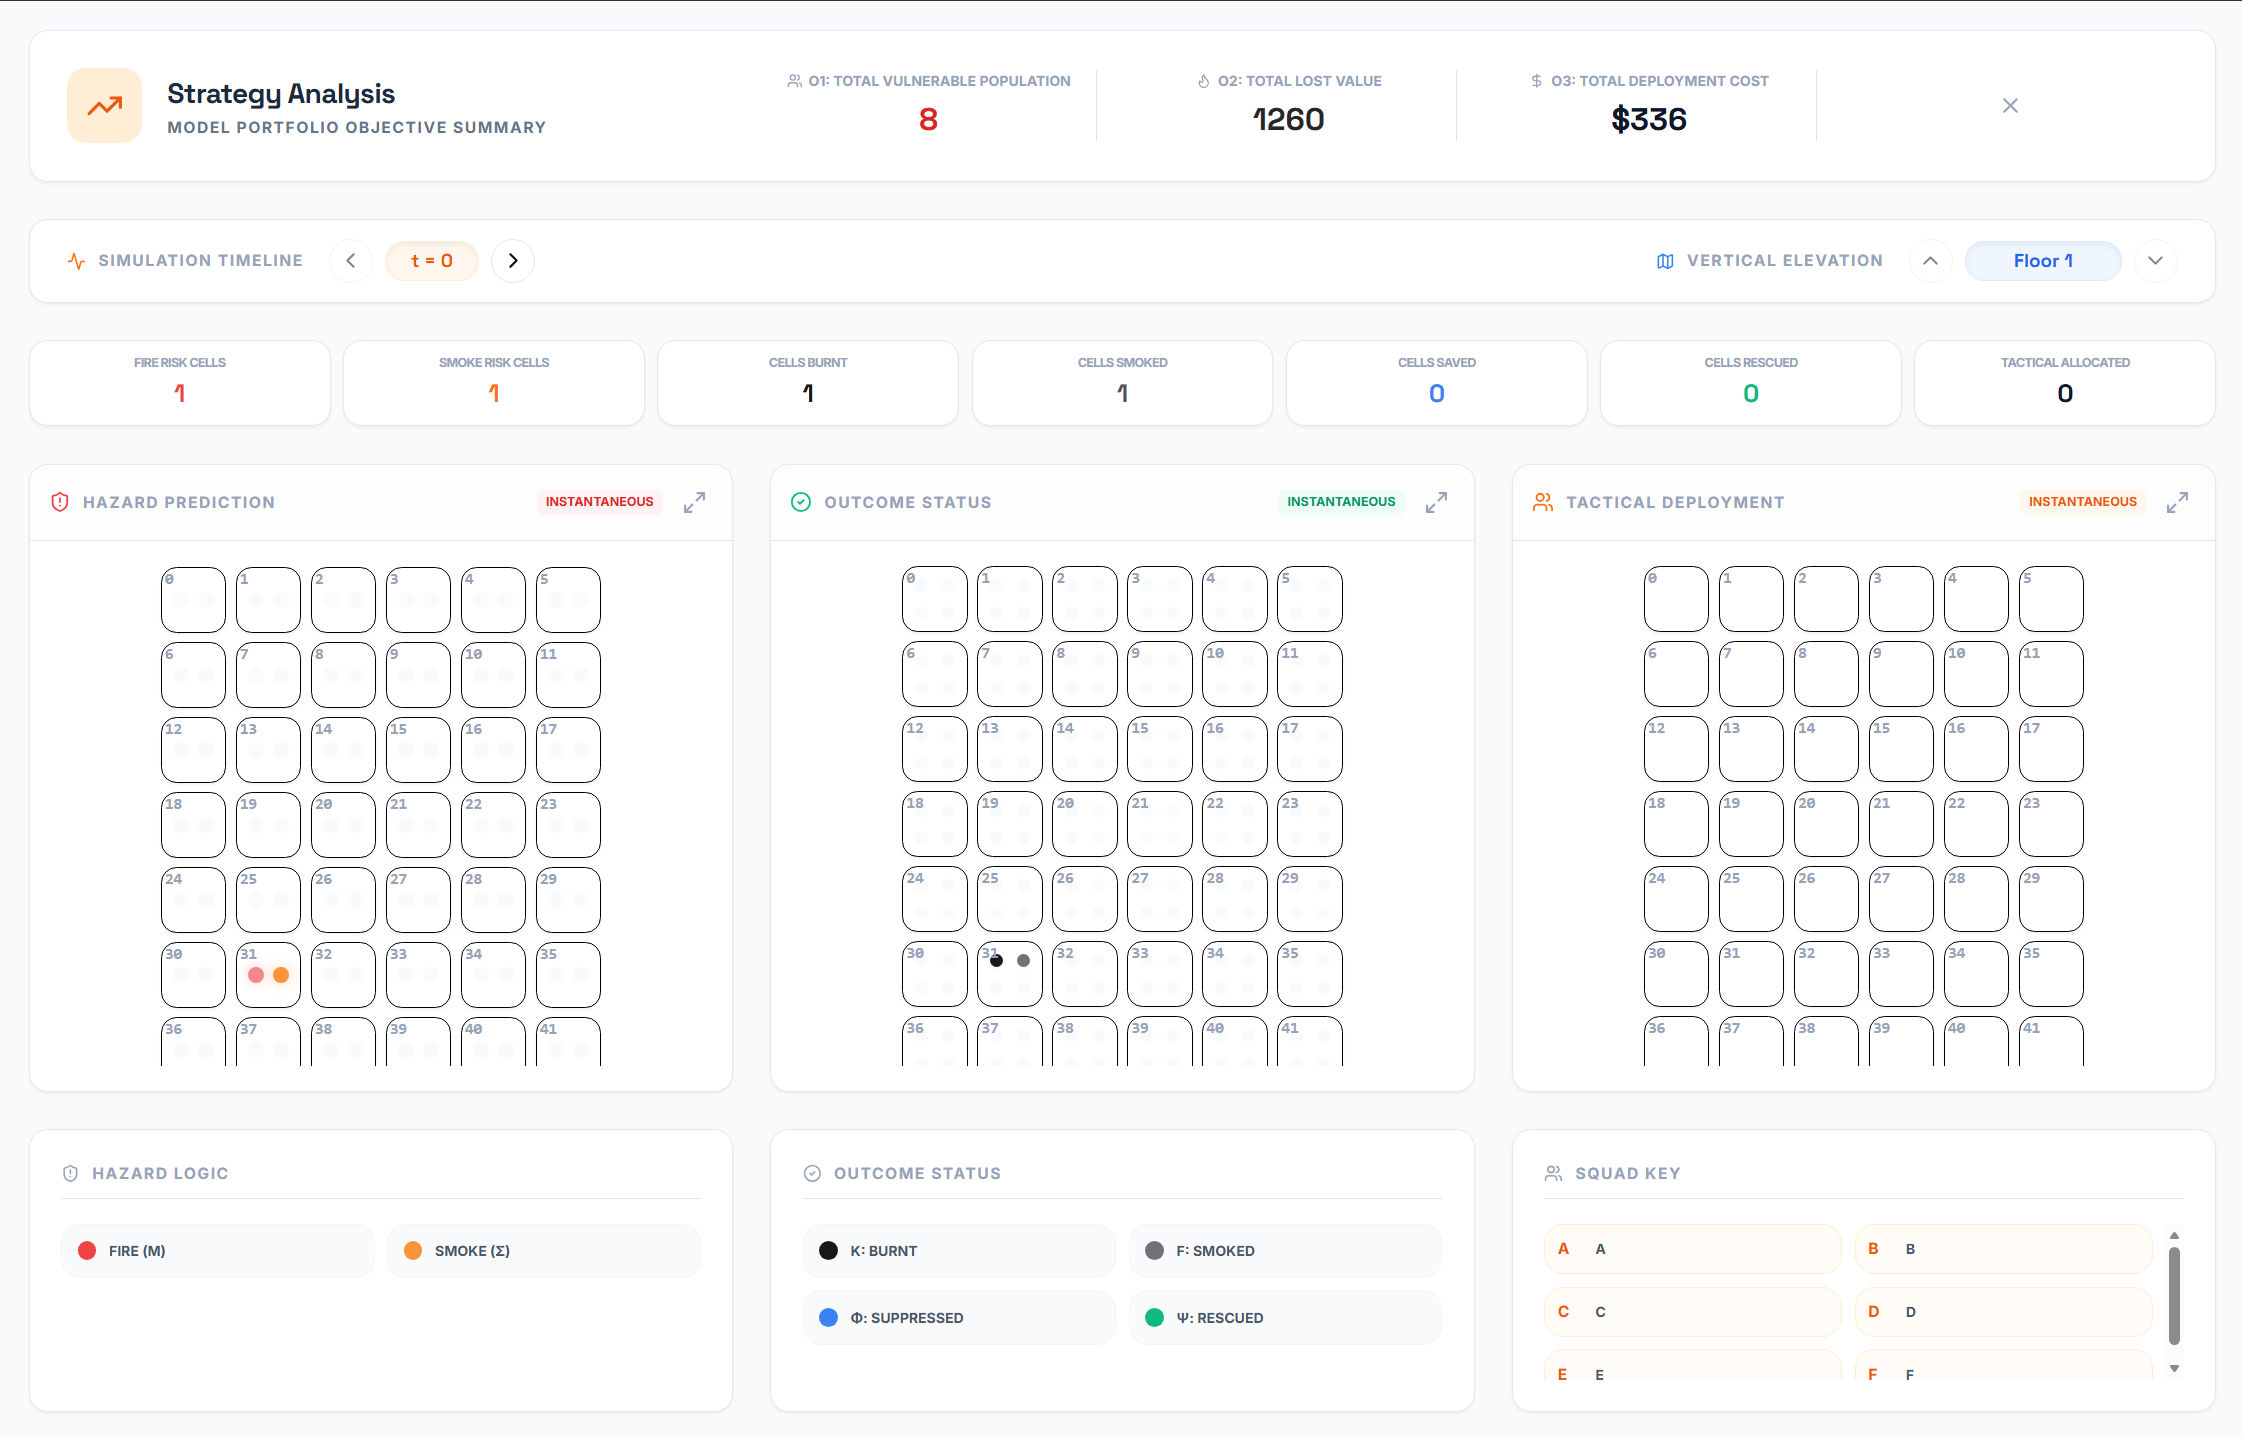
\includegraphics[width=0.32\textwidth]{figures/3t0.png}}
\hfil
\subfloat[$t=1$]{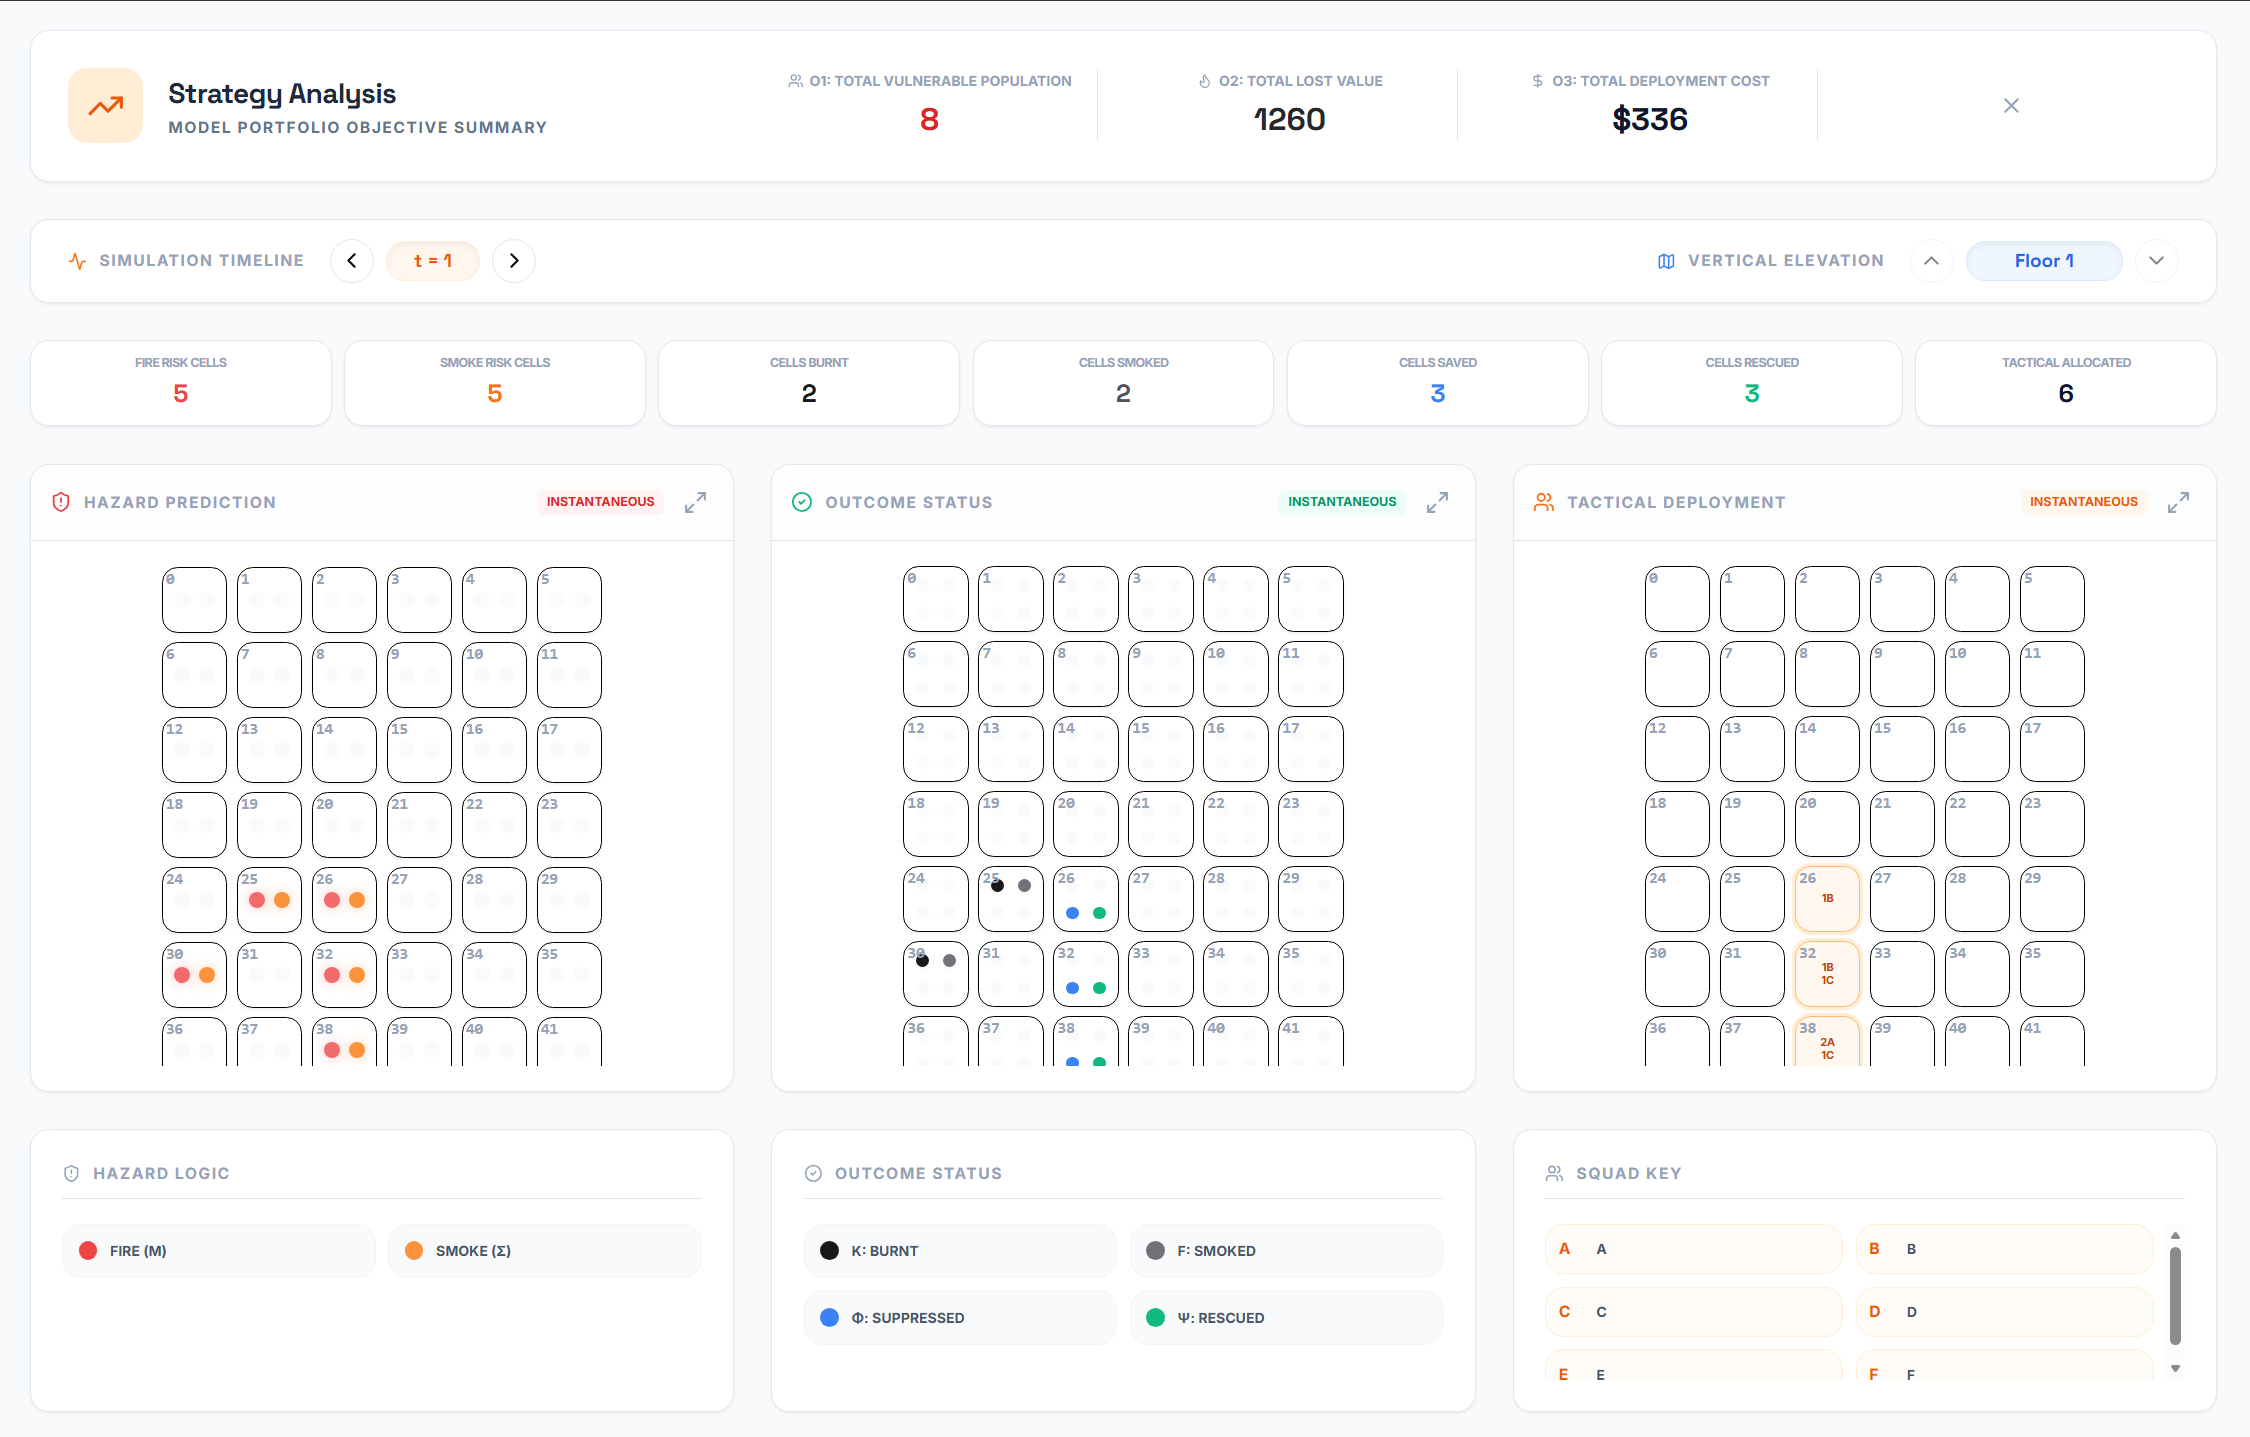
\includegraphics[width=0.32\textwidth]{figures/3t1.png}}
\hfil
\subfloat[$t=2$]{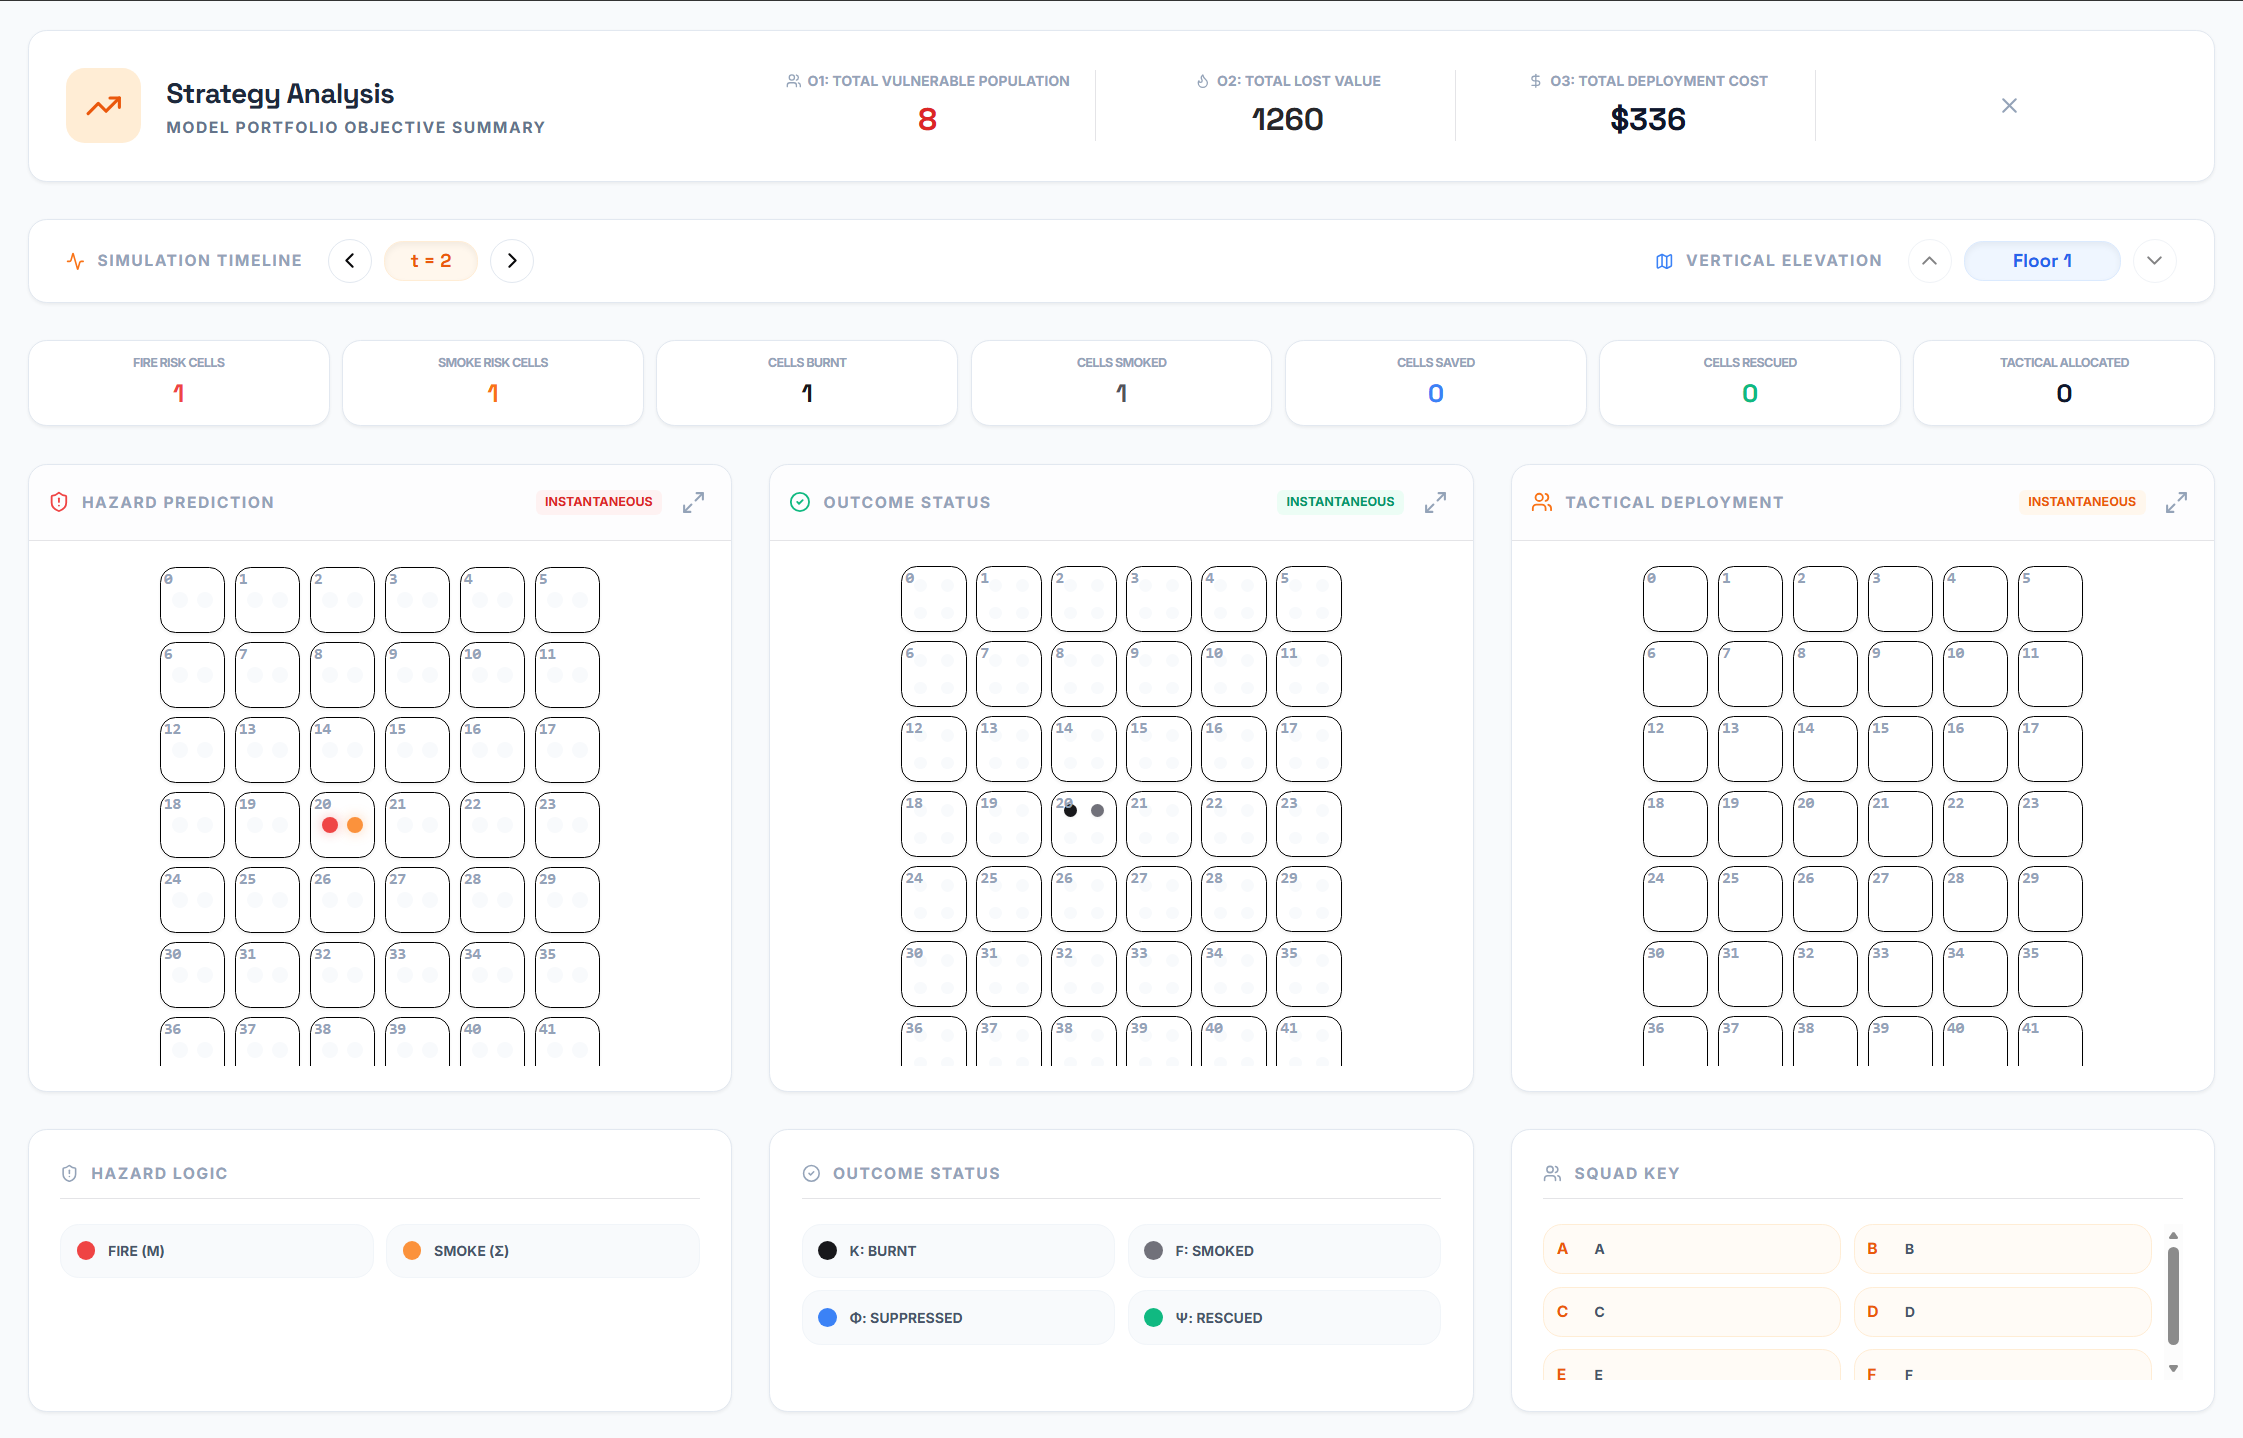
\includegraphics[width=0.32\textwidth]{figures/3t2.png}} \\
\subfloat[$t=3$]{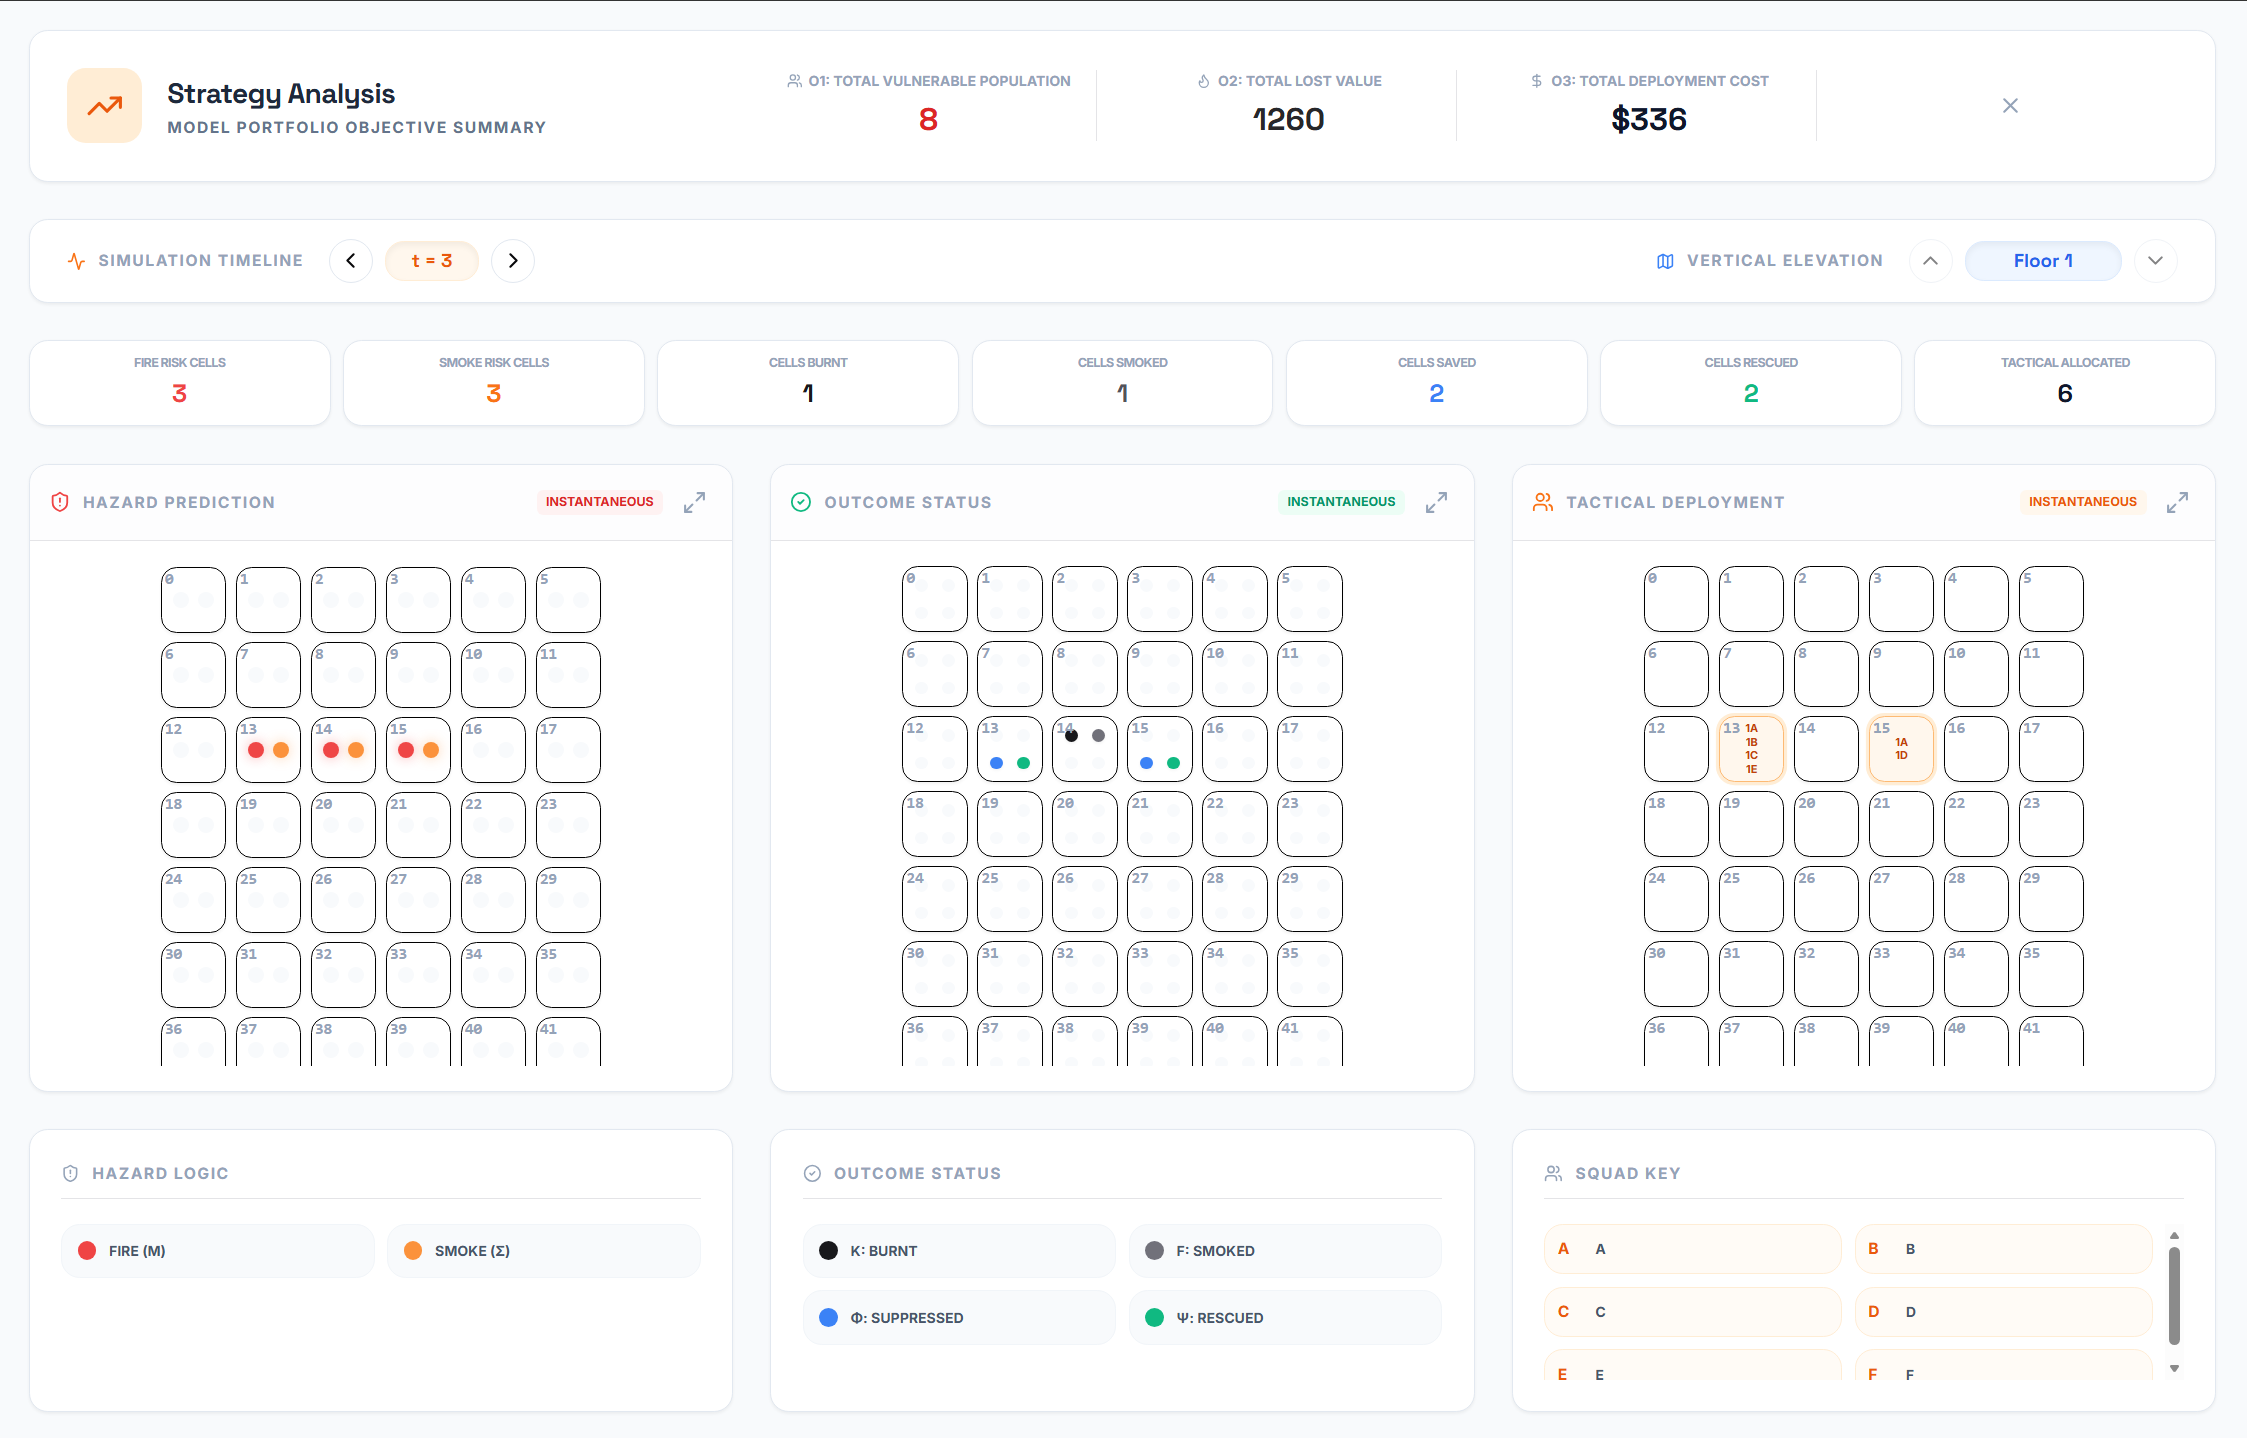
\includegraphics[width=0.32\textwidth]{figures/3t3.png}}
\hfil
\subfloat[$t=4$]{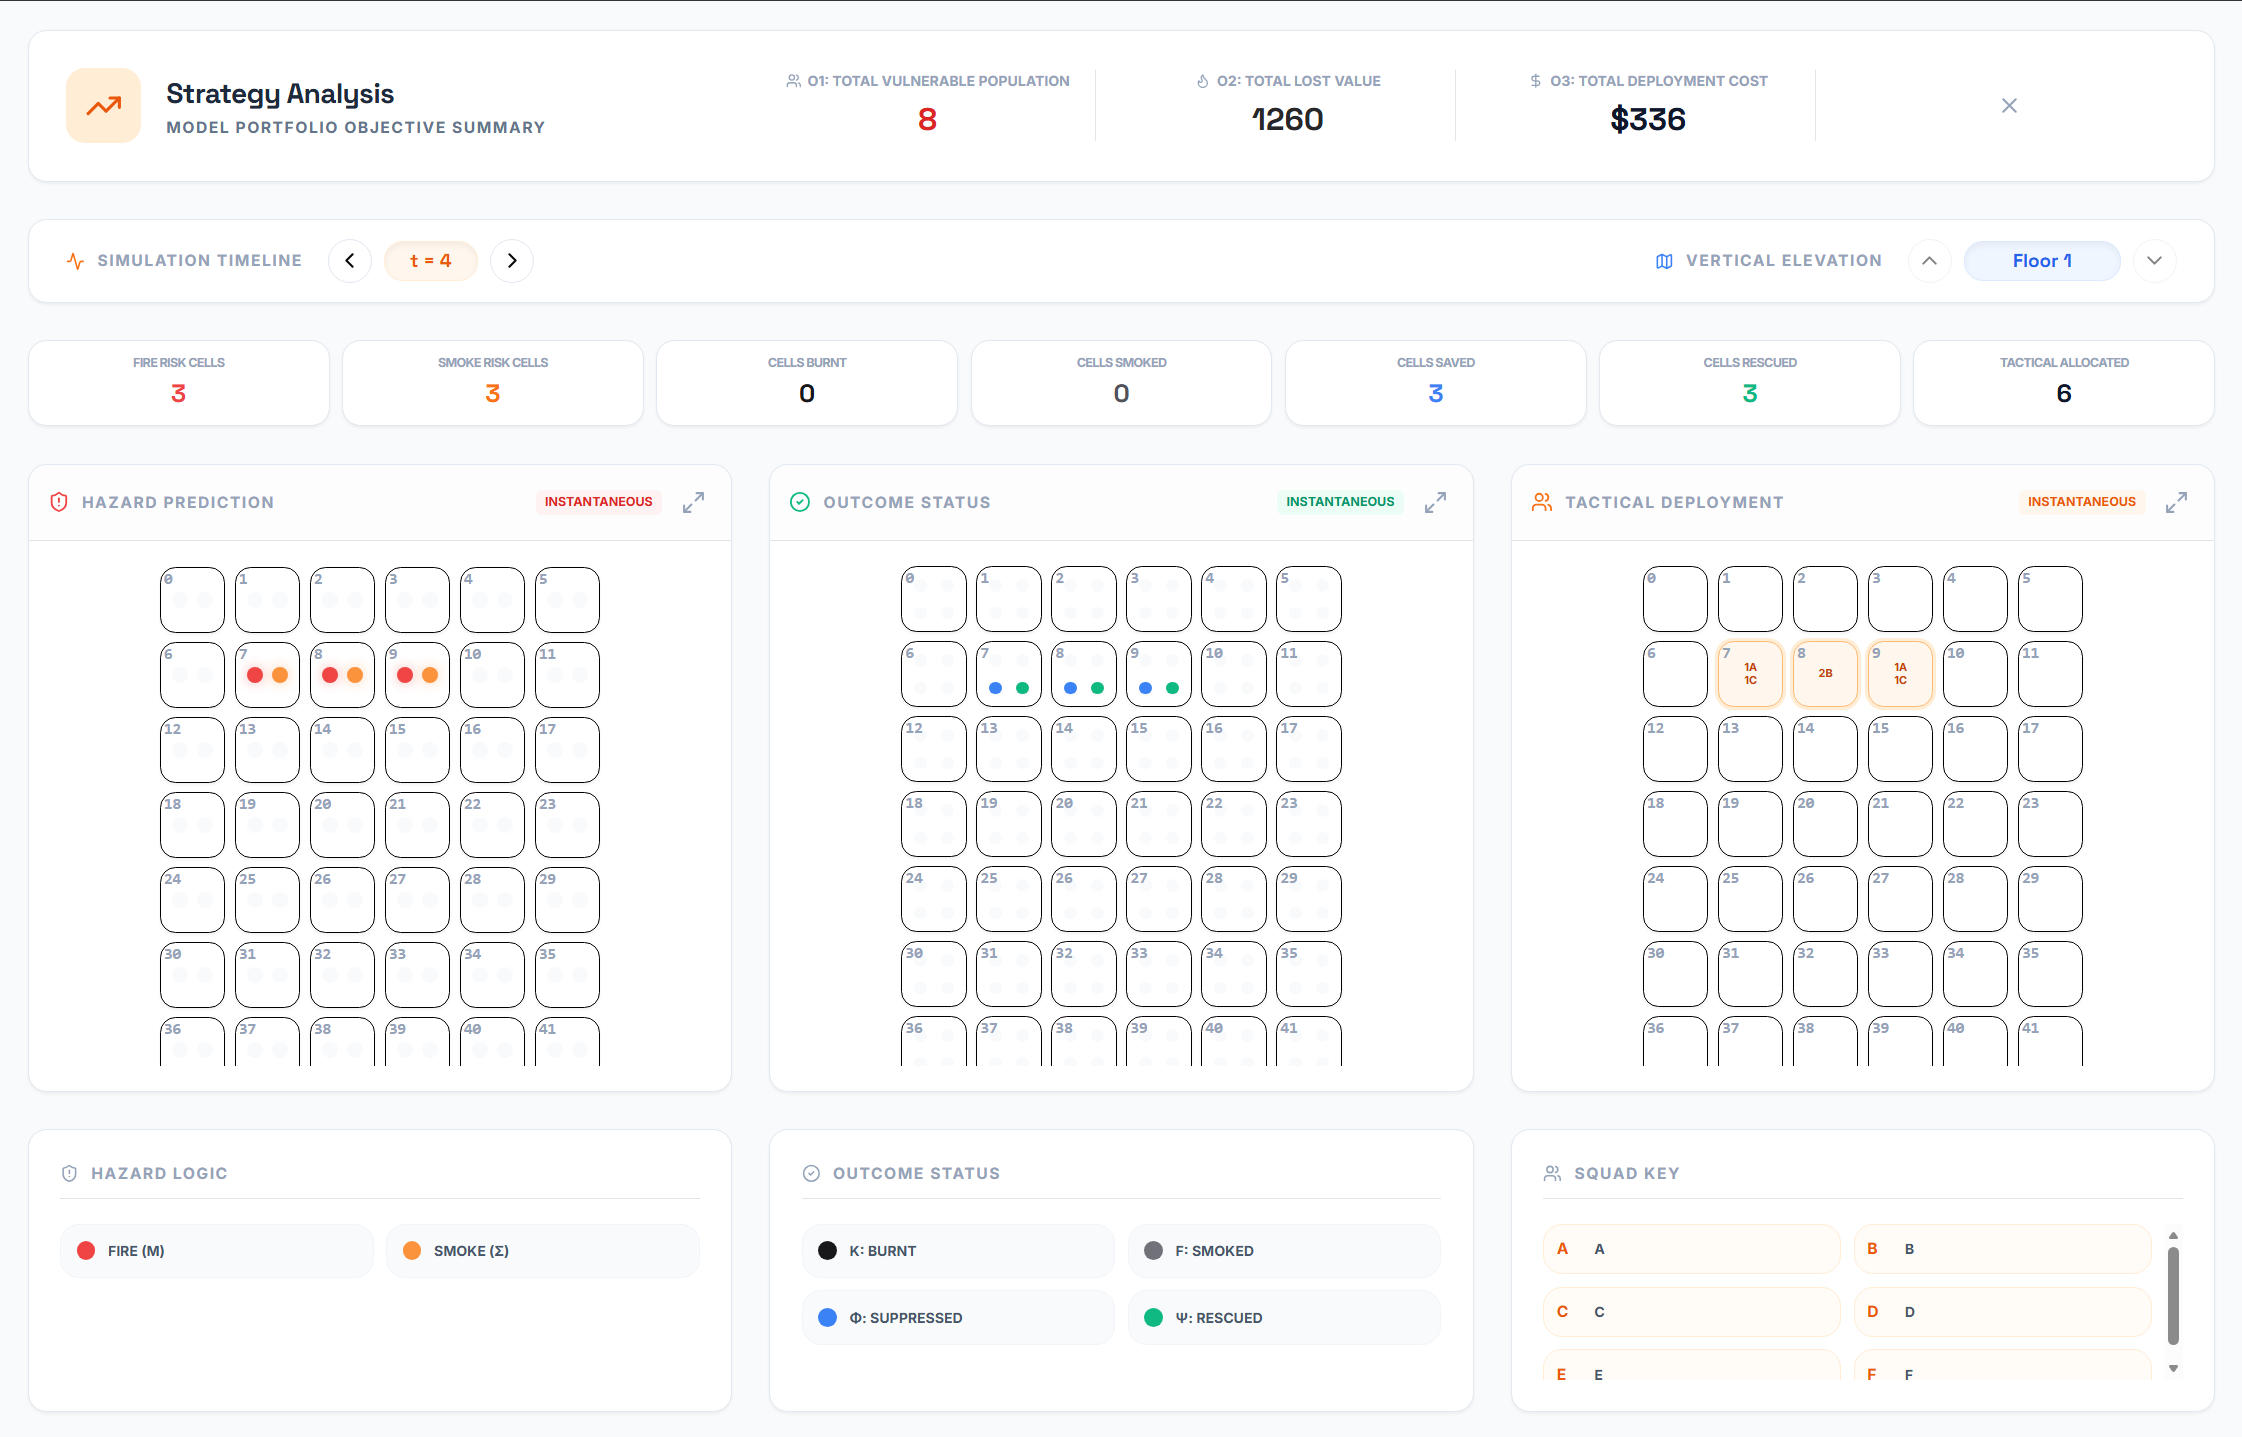
\includegraphics[width=0.32\textwidth]{figures/3t4.png}}
\caption{Optimal deployment strategies: hazard prediction, outcome status, and tactical allocation across time steps.}
\label{fig:simulation-results}
\end{figure*}

\clearpage